\hypertarget{sec:awsm-ci}{%
\chapter{AWSM Customer Impact Control Method}\label{sec:awsm-ci}}

This chapter addresses research objective \cref{ro:3}:

\vspace{-5pt}
\begin{quote}
To enable control of the impact of user interface changes through \gls{Web Migration} on customers with limited resources and lack of \gls{Web Engineering} expertise.
\end{quote}
\vspace{-5pt}
First, three research questions are derived from \cref{ro:3}, and the current situation is briefly analyzed to identify requirements and review related work.
To address the research questions, two sections outline the two main contributions towards \cref{ro:3} in the context of the AWSM:CI method: the concept of Visual Analysis of \gls{ui} Similarity for customer impact control is introduced including a model for computation of similarity and a process for calibrating the similarity computation, and a technique for automatically detecting user interface elements is presented.
Finally, the method is evaluated against the requirements, and the evaluation is supported by empirical experimentation.

\vspace{-30pt}
\hypertarget{sec:ci.analysis}{%
\section{Analysis}\label{sec:ci.analysis}}
\vspace{5pt}

The following analysis briefly summarizes the situation of customer impact through visible changes in the user interface caused by \gls{Web Migration} and the challenges of measuring the similarity of user interfaces for controlling the customer impact.
Requirements are derived from this analysis and an overview of related work on the two enabling fields of research used for AWSM:CI is given.

\subsection{Situation and Challenges}
\vspace{10pt}

\glspl{isv}, as described in \cref{sec:scenario}, have accumulated large userbases, with long-running customer relationships and contracts for updates and maintenance, that are familiar with the \gls{Legacy System} and well-adapted to its \glslink{Legacy System}{legacy} user interface.
Adaption can extend up to the business process level: we observed that the business processes in many doctors' offices are governed by the processes represented in the \gls{pms} (cf. \cref{sec:research-process}).
This makes it hard to introduce changes in user interaction or even replace the \gls{pms} because of the potential \emph{customer impact} (cf.~\cref{fig:problem-tree}).
In industry contexts, it is therefore often a requirement to limit differences and maintain the \emph{look and feel} of the \glslink{Legacy System}{legacy} user interface to avoid forcing end users to change their working habits \autocite{Lucia2008,Lucia2006,Distante2002}.
Customers often ``require new applications to look like the old ones through similar screens and interaction ways even if new applications are Web-based'' \autocite{Remics2013RecoverToolkit}.
%In the \gls{Forward Engineering} phase of a traditional horseshoe reengineering approach, it is ``important to comply with the cognitive characteristics of the legacy application'' \autocite{Distante2006a}.
Learning how to use a new \gls{web} user interface requires an effort for customers.%, which \gls{isv} customers are not immediately willing to take.
Thus changing the \gls{ui} poses a risk for the \gls{isv}. % as it can mean, in the worst case, to lose customers.
%The awareness of this risk contributes to intra-organisational resistance \autocite{Khadka2014ProfessionalsModernization}.

\gls{Web Migration} visibly impacts the user interface and, therefore, its users.
The \glslink{Legacy System}{legacy} \gls{ui} consists of windows, rendering controls according to the \glslink{Desktop Application}{desktop} \gls{gui} framework and platform. % in use.
A \gls{web} \gls{ui}, in contrast, is rendered in a \gls{web} browser in browser tabs, rendering controls according to the \gls{web} \gls{ui} framework, platform, and specific \gls{css} styles.
%Changing the \glslink{Legacy System}{legacy} interaction paradigm towards a navigational paradigm is one of the most critical challenges of \gls{Web Migration} \autocite{Distante2002}.
The industry requirement of maintaining a similar look and feel causes the challenge of \emph{\gls{ui} Similarity}.
Analysis of \gls{ui} Similarity is a research area of \gls{hci}, application of which exceeds \gls{Web Migration}, supporting testing, cross-platform \gls{gui} matching, \gls{gui} modernization, and project effort estimation \autocite{Grechanik2018}.

To ``avoid presenting the user with a drastically different application'' \autocite{Distante2006a}, changes need to be controlled, favoring an incremental transition evolving the software over abrupt changes (cf.~also \cref{fig:problem-tree}).
Design decisions concerning the user interface need to be informed through \gls{ui} Similarity Analysis.
Changes that affect \gls{ui} Similarity can occur in several dimensions: \emph{Task} \autocite{Bakaev2017WebIntelligence,Stroulia2002}, i.e.~the workflow required to achieve a specific user goal on the \gls{ui}, \emph{Behavior} \autocite{Stroulia2002}, i.e.~the way the user interacts with the user interface, \emph{Thesaurus}, i.e.~the textual vocabulary used in the user interface for labels etc.
and the visual vocabulary such as icons, images etc., \emph{Layout}, i.e.~how \gls{ui} controls are placed and sized, and \emph{Material}, i.e.~how \gls{ui} Elements look like \autocite{Bakaev2017Kansei}.
%The goal is to ``preserve the old (established) mode of operation \emph{as far as possible}'' \autocite{Distante2006a}.
\gls{ui} Similarity in the context of \gls{Web Migration} focuses on dimensions in which changes cannot be avoided, to allow for an informed choice within the degrees of freedom of the \gls{ui} design space. 
%This possibility defines the target scope for \gls{ui} Similarity in the context of \gls{Web Migration}: it focuses on dimensions in which changes cannot be avoided, to allow for an informed choice within the degrees of freedom of the \gls{ui} design space.

%In the specific context of \gls{Web Migration}, not all dimensions of \gls{ui} Similarity are equally important.
%Changes of Thesaurus such as renaming elements or Task, i.e.~modifying the business processes, can and should be avoided \autocite{Sneed2010SoftwareMigration,Sneed1995CostBenefit} during \gls{Web Migration}.
Changes in Layout and to some degree in Behavior and Material follow conclusively from the \emph{change of environment} through \gls{Web Migration}.
Layout changes result from the different layout paradigms (pixel-based/grid-based, cf.~\cref{sec:uitransformation}), material changes (\gls{gui} framework  controls/\gls{css}-styled controls), and viewing conditions (fixed-size desktop window/variable-sized browser window), which cause changes in the positioning and size of \gls{ui} controls.
Positions and sizes of controls define the degrees of freedom of the design space for creating a \glslink{web}{Web}-based version of a \glslink{Legacy System}{legacy} \gls{ui}.
As Layout describes the visual organization of content, it provides orientation for the user and has a considerable impact on the Behavior dimension.
Thus, similarity of Layout is particularly relevant for \gls{ui} Similarity in the context of \gls{Web Migration}. %: capturing the \glslink{Legacy System}{legacy} \gls{ui} layout is a ``preponderant requirement'' of \glslink{Software Modernization}{modernization} to regenerate the \glslink{Legacy System}{legacy} look and feel \autocite{Rodriguez-Echeverria2012MIGRARIA}.

\emph{Measurability} is necessary to quantify the state of \glspl{Legacy System} \autocite{Masak2006}.
However, existing \glslink{Legacy System}{legacy} metrics are focused on the \gls{Legacy System} only and do not consider \glslink{target system}{target} and \gls{source system} together.
To control the customer impact of user interface \gls{ui} changes through \gls{Web Migration}, changes affecting \gls{ui} Similarity must be made measurable.
%The importance of measurement for engineering in general and software engineering in particular is widely acknowledged \autocite{SWEBOK2014}.
Existing \gls{Web Migration} approaches as in \cref{sec:approaches} barely consider \gls{ui} Similarity beyond an abstract level, without providing a concrete way of measuring it.
%Existing \gls{Web Migration} approaches as in \cref{sec:approaches} barely consider \gls{ui} Similarity, often referred to as a similar ``look and feel'' \autocite{Rodriguez-Echeverria2012MIGRARIA,Lucia2008,Lucia2006}, beyond an abstract level, without providing a concrete way of measuring it. %, or for \glspl{tui} only \autocite{Bodhuin2002DesktopWebMVC} which have a significantly reduced design space.
%
Existing \gls{ui} Similarity Analysis approaches cannot be applied to \glslink{Legacy System}{legacy} and \gls{web} \glspl{ui} because they are based on code analysis or target a different degree or dimension of similarity.
Measurement of \gls{ui} Similarity is therefore not directly applicable to \gls{Web Migration} and needs to be adapted to the characteristics of migration and the situation of \glspl{isv} with non-\glslink{web}{Web} \glslink{Legacy System}{legacy} \glslink{Desktop Application}{desktop software}.

\vspace{-5pt}
Thus, the challenge is to specify a suitable customer impact method for measuring the \gls{ui} Similarity between the \glslink{Legacy System}{legacy} \gls{ui} and \glslink{web}{Web}-based versions of the \gls{ui} that can be used to inform design decisions, control the amount of changes introduced and incrementally evolve the user interface towards a modern \gls{web} user interface with limited resources and \gls{Web Engineering} expertise.

\vspace{-18pt}
\hypertarget{sec:ci.requirements}{%
\subsection{Requirements}\label{sec:ci.requirements}}
\vspace{6pt}

The following requirements specify \cref{ro:3}, based on the analysis presented above and the \gls{awsm} principles.

\vspace{-10pt}
\textbf{Effectiveness}. Customer impact control of \gls{Web Migration} should be enabled through measurement of \gls{ui} Similarity between \glslink{Legacy System}{legacy} and \gls{web} user interfaces.

\vspace{-10pt}
\textbf{Efficiency}. Measurement of \gls{ui} Similarity should be supported by analysis tools to automate the measurement process.

\vspace{-10pt}
\textbf{Expertise}. Measurement of \gls{ui} Similarity should be feasible with available expertise of the \gls{isv}'s staff.

\vspace{-10pt}
\textbf{Applicability}. Measurement of \gls{ui} Similarity should be applicable to a wide range of \glslink{Legacy System}{legacy} and \gls{web} user interfaces, including user interface design prototypes (\gls{ui} mockups), independent of the specific \gls{ui} technology.

\vspace{-10pt}
\textbf{Calibratability}. \gls{ui} Similarity measurement results should be calibratable to the perceptual characteristics of specific customer target groups.

\vspace{-42pt}
\hypertarget{sec:ci.related-work}{%
\subsection{Related Work}\label{sec:ci.related-work}}
\vspace{7pt}

This section introduces \gls{ui} Layout Similarity Analysis and Analysis of \gls{ui} Structure as key research areas enabling the AWSM:CI method.
It establishes the semantics of the terminology and the blueprint strategies used in the following description of AWSM:CI and provides a minimal overview of related work in both fields.

\textbf{\gls{ui} Layout Similarity Analysis} is an active field of research, comprising GUI Differencing and Cross-Browser Inconsistencies detection.
\emph{\gls{gui} Differencing} \autocite{Grechanik2018,Grechanik2009ICSE,Grechanik2009ICSM} focuses on automatic \gls{gui} test script adaption after maintenance activities changing the \gls{gui}.
Automated \emph{sound} (precision=1) and \emph{complete} (recall=1) \gls{gui} differencing is \emph{undecidable} \autocite{Grechanik2018}.
\emph{\gls{xbi} detection} is the automatic detection of layout variations of \gls{web} \glspl{ui} rendered in different browsers/mobile platforms/viewports.
Most approaches follow a \emph{\gls{dom}-based strategy} \autocite{Watanabe2018,RoyChoudhary2014XPERT,RoyChoudhary2010WebDiff}, requiring the \gls{dom} for segmentation of the \gls{wui} or identification of \glspl{xbi}.
\emph{Computer-vision strategies} \autocite{Saar2016Browserbite} work based on analysis of \gls{wui} screenshots.
\emph{WebDiff} \autocite{RoyChoudhary2010WebDiff} introduced the blueprint two-step \emph{differential testing} \autocite{Mckeeman1998DifferentialTesting} strategy followed by many \gls{xbi} approaches: 1) segmentation of the \gls{wui} according to its \gls{dom} structure and 2) comparisons of corresponding \gls{ui} controls across the different versions of the user interface.

Both \gls{gui} Differencing and \gls{xbi} detection analyze \gls{ui} Layout Similarity, \gls{gui} Differencing within a fixed environment, i.e.~on the same platform and framework, XBI detection within different \gls{html} rendering engines.
However, the \gls{ui} Layout variations are more subtle compared to the consequences of migration from a \glslink{Desktop Application}{desktop} \gls{gui} to the \gls{web}: \gls{gui} Differencing addresses intended \gls{ui} changes through perfective maintenance activities, \gls{xbi} detection addresses even more subtle unintended changes through rendering differences of a \gls{wui} with identical description.
While \gls{ui} Similarity Analysis for \gls{Web Migration} requires a similar matching of \gls{ui} controls across different \gls{ui} versions, these changes are more coarse-grain and prominent.
Thus, the aspect of subjective perception of similarity is more important in contrast to the detection of fine-grain \gls{ui} changes for \gls{gui} Differencing or \gls{xbi} detection.
%Smaller and fewer differences allow for higher precision \autocite{Grechanik2018}.

\textbf{Analysis of \gls{ui} Structure} is an important pre-requisite for \gls{ui} Analysis to identify the visually and semantically coherent two-dimensional segments, that constitute the \gls{ui}.
\gls{ui} controls form atomic segments of a \gls{ui} and create a hierarchy through containment and alignment relationships \autocite{Choudhary2013XPERT}.
\emph{Page Segmentation} approaches address the problem of identification of segments in \glspl{wui} and are employed in \gls{web} data extraction, crawling, archiving, accessibility, visual quality evaluation, and automatic page adaption or retargeting \autocite{Sanoja2014,Talton2011Bricolage,Liu2010VIDE,Cai2003VIPS}.
The majority of approaches require the \gls{dom} as input for segmentation, which is not available for the \glspl{source system} of \gls{Web Migration}.
\emph{Vision-based Segmentation} approaches like \autocite{Kong2012} instead apply image processing for recognition of atomic interface objects.
This requires two activities: segmentation into candidates, called \glspl{roi}, using edge detection and analysis of geometric shapes, and classification of \gls{gui} Element type or rejection of the candidate.
Other vision-based strategies like Sketch2Code\footnote{\url{https://sketch2code.azurewebsites.net/} Retrieved: 6.12.2019}, AirBnB's Sketching tool\footnote{\url{https://airbnb.design/sketching-interfaces} Retrieved: 6.12.2019}, and pix2code\footnote{\url{https://github.com/tonybeltramelli/pix2code} Retrieved: 6.12.2019} focus on the generation of \glspl{ui} from hand-drawn \gls{ui} mockups through analysis of \gls{ui} objects.
While they provide strong examples of the power of computer-vision based approaches and the use of Artificial Intelligence (AI) in \gls{ui} Similarity, our experiments could not produce any useable results when using \glslink{Legacy System}{legacy} \gls{gui} screenshots\footnote{a sample result for a legacy interface used in our own evaluation experiments \autocite{Heil2016Similarity} is available here: \url{https://sketch2code.azurewebsites.net/generated-html/350d13fa-6bf3-43e4-9e6d-04a58d77bb0c} Retrieved: 6.12.2019}.

Consideration of \emph{\gls{ui} Similarity in \gls{Web Migration}} is sparse.
The few approaches which do, fail to provide a concrete way of measuring it \autocite{Remics2013RecoverToolkit,Rodriguez-Echeverria2012MIGRARIA,Lucia2008,Distante2006a}, focus on interactions, i.e.~the Behavior and Task dimension of \gls{ui} Similarity \autocite{Cajas2019}, disregarding layout and visual aspects, are targeting \glslink{Legacy System}{legacy} systems with \glspl{tui} \autocite{Stroulia2003,Bodhuin2002DesktopWebMVC} or which have already \glspl{wui} \autocite{Lucia2007SimilarPages} and do only use static page structure information, falling significantly behind the state of the art in other fields like \gls{xbi} detection or page segmentation.

Due to the independence of computer-vision-based strategies for  \gls{ui} Similarity Analysis from heterogeneous textual representations of \glspl{ui}, \cref{sec:visual-analysis} describes the application of computer-vision to \gls{ui} Similarity Analysis in \gls{Web Migration} by specification of a technique for measuring the similarity between the similarity of layouts between \glslink{Legacy System}{legacy} non-\glslink{web}{Web} and \gls{web} versions of graphical user interfaces throughout \gls{Web Migration} with limited resources and lack of \gls{Web Engineering} expertise.
%The following section introduces the computer-vision-based \gls{ui} Similarity Analysis of AWSM:CI.

\hypertarget{sec:ci.research-questions}{%
\section{Research Questions}\label{sec:ci.research-questions}}
\vspace{15pt}

The analysis presented above raises three research questions:

\begin{quote}
\textbf{AWSM:CI Research Question RQ1}: How to control the impact of \gls{Web Migration} on customers with limited resources and lack of \gls{Web Engineering} expertise?
\end{quote}

\begin{quote}
\textbf{AWSM:CI Research Question RQ2}: How to measure the similarity of non-\glslink{web}{Web} and \gls{web} versions of a user
interface?
\end{quote}

\begin{quote}
\textbf{AWSM:CI Research Question RQ3}: How to analyze visual \gls{ui} Similarity through computation of objective measurements?
\end{quote}

To design and evolve a solution for research objective \cref{ro:3}, this chapter addresses these three research questions in the following sections.

\vspace{-15pt}
\hypertarget{sec:visual-analysis}{%
\section{UI Similarity Analysis}\label{sec:visual-analysis}}
\vspace{15pt}

To enable the control of the impact of user interface changes caused by \gls{Web Migration} on existing customers set as research objective \cref{ro:3}, AWSM:CI allows to measure the visual similarity between \legacy and \web user interfaces.
Addressing the resources and expertise constraint of \cref{ro:3}, AWSM:CI defines a technique for computation of similarity based on objective measures and a tool for automatic detection of user interface elements.
It provides an answer to AWSM:CI RQ1.
\Cref{sec:visual-analysis.overview} provides an overview of the method, \cref{sec:calibration} specifies a technique for calibration of the method to target user groups, \cref{sec:computing-sim} describes the computation of similarity and \cref{sec:ci.integration} addresses integration of the method with ongoing development activities of \glspl{isv}.

\hypertarget{sec:visual-analysis.overview}{%
\subsection{Visual Analysis of UI Similarity}\label{sec:visual-analysis.overview}}
\vspace{5pt}

For analyzing visual similarity of user interfaces in \gls{Web Migration}, a computer-vision based approach is required.
This section addresses the challenge of specification of a computer-vision approach for User Interface Similarity Analysis, answering AWSM:CI RQ2.

\emph{Visual \gls{ui} Similarity Analysis} in the context of \gls{Web Migration} aims at measuring the similarity between the non-\glslink{web}{Web} \glslink{Legacy System}{legacy} \gls{gui} \(u_{legacy}\) and the \glslink{web}{Web}-based versions of the \gls{gui} \(\{u_{web,1}, \ldots, u_{web,n}\}\) created throughout \gls{Web Migration} based on \emph{visual aspects} \autocite{Heil2016Similarity,Bakaev2017Kansei}.
These visual aspects are \emph{features} \(x_i\) defined through \emph{feature engineering} for a \emph{design mining} process \autocite{Bakaev2017WebIntelligence} and used as vector components for a \emph{vector-space representation} \(\vec x_u \in \mathbb{R}^d\) of \gls{ui} \(u\) required for comparison and classification.
Calculation of similarity measurements is based on these features, identifying \emph{regions of interest} \(R_u=\{r_1, \ldots, r_l\}\), and extracting visual features for these regions.
AWSM:CI defines two categories of features: \emph{atomic features} \autocite[equivalent to \emph{base measures}][]{ISO/IEEE2017Measurement} which can be assessed per \gls{ui} independently such as density \autocite{Heil2016Similarity} or complexity \autocite{Bakaev2017Kansei} and \emph{relative features} \autocite[equivalent to \emph{derived measures}][]{ISO/IEEE2017Measurement} which are assessed on a pair of user interfaces and describe differences such as order or orientation \autocite{Heil2016Similarity}.

These two feature types closely relate to different levels of \gls{ui} Similarity.
Atomic features require a lower structural and content similarity than relative features.
For instance, complexity can be assessed of two arbitrary \glspl{ui} and compared, whereas changes in order can only be assessed on a pair of \glspl{ui} sharing a common subset of \gls{ui} controls.
\gls{gui} Differencing and XBI detection focus on a very narrow notion of similarity of \gls{ui} versions with little to no changes based on relative features such as position and size changes.
A design repository and search engine like Webzeitgeist \autocite{Kumar2013Webzeitgeist}, on the other hand, requires a wide notion of similarity to be applicable to arbitrary \glspl{ui} mainly based on atomic features such as GIST features \autocite{Oliva2001GIST}.
\gls{Web Migration} is located between these two extremes: the \gls{ui} differences are higher than between versions of the same \gls{ui} (\gls{gui} Differencing) or \glspl{wui} rendered in different browsers (XBI detection), but lower than between arbitrary \glspl{ui} (Design Search Engines) and \glslink{Legacy System}{legacy} and \glslink{web}{Web}-based \gls{ui} share a common subset of controls.
Thus, \gls{ui} Similarity in the context of \gls{Web Migration} requires both atomic and relative features.
Based on these features, a \emph{similarity function}

\begin{equation}sim: \mathbb{R}^d \times \mathbb{R}^d \mapsto \mathbb{R}\label{eq:sim}\end{equation}

can be calculated.
%, similar to the metric learning approach in OASIS \autocite{Chechik2010OASIS}.
%However, an image-based similarity using edge and color histogram comparisons is not applicable due to the conclusive differences particularly in the \emph{Material} dimension of similarity and the non-hold of its \emph{relevance sparsity assumption}: assuming a relevance score of zero for unknown combinations makes sense for arbitrary image comparisons, but not for comparisons between non-\glslink{web}{Web} and \gls{web} versions of the same \gls{gui}.
%Instead, the 
The similarity function \(sim\) needs to be an approximation of \emph{perceived \gls{ui} Similarity} \(\mathfrak{S}\), which is influenced by subjective cognitive aspects \autocite{Bakaev2017Kansei} and semantic structure of the \gls{gui}:

\begin{equation}\mathfrak{S}: U \times U \mapsto \in \mathbb{R}\label{eq:perceived-sim}\end{equation}

\gls{ui} Similarity is still an active field of research and perceived \gls{ui} Similarity \(\mathfrak{S}\) is not yet well understood.
\(\mathfrak{S}\) can be empirically measured, e.g.~as we demonstrated using a set of \emph{Kansai scales} \autocite{Bakaev2017Kansei} and pair-wise comparisons.
Yet, empirical measurement requires test subjects from the target user group, i.e.~the \gls{isv}'s customers in \cref{sec:scenario}.
If a similarity function \(sim\) calculated from feature vectors is indicative of \(\mathfrak{S}\), then it can be used to replace tedious empirical comparisons of \gls{ui} pairs in \gls{Web Migration} and thus facilitate predicting perceived similarity compared to manual assessment.
For \(sim\) to perform as approximation of \(\mathfrak{S}\), at least a \emph{concordant} (positive monotonic) relationship is required, i.e.~an arbitrary (but unknown) monotonic function can describe the relationship between \(\mathfrak{S}\) and \(sim\) for larger sample sets (\emph{generalization assumption}):

\begin{equation}sim(\vec x_u, \vec x_{u^+}) > sim(x_u, \vec x_{u^-}) \implies \mathfrak{S}(u, u^+) > \mathfrak{S}(u, u^-)\label{eq:sim-assumption}\end{equation}

That means that \emph{Visual \gls{ui} Similarity Analysis for \gls{Web Migration}} is a process of constructing a similarity function \(sim\) based on vector-space representations of two user interfaces derived from visual features, that is indicative of perceived \gls{ui} Similarity \(\mathfrak{S}\).
The conceptual model of this process is shown in \cref{fig:ci-process}.

\begin{figure}[h!]
\hypertarget{fig:ci-process}{%
\centering
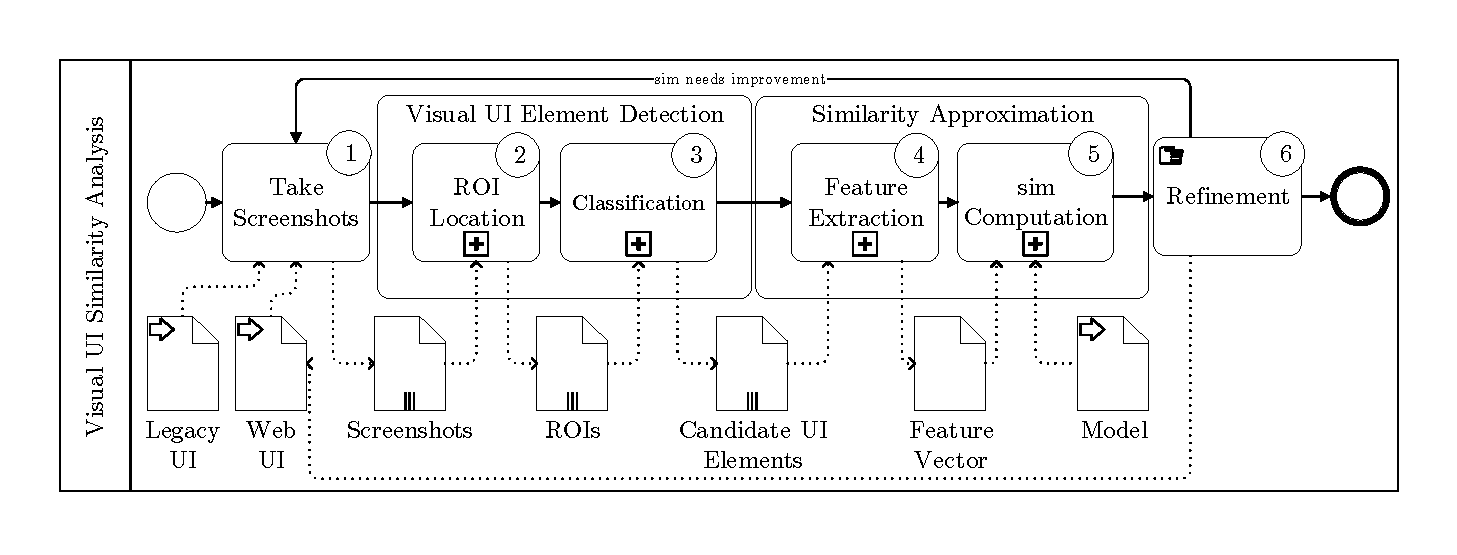
\includegraphics[width=0.99\textwidth]{../figures/awsm-ci-process.pdf}
\caption{Visual UI Similarity Analysis Process}\label{fig:ci-process}
}
\end{figure}
The process follows a visual bottom-up version of the WebDiff strategy, starting with screenshots of both \glspl{ui} in (1), the Visual \gls{ui} Element Detection phase, which consists of locating \glspl{roi} (2) and classification (3), followed by the similarity approximation phase based on feature extraction (4) and computation of \(sim\) (5) which can be then used to drive design decisions and refine (6) the \gls{wui} and repeat the cycle.

This process defines the AWSM:CI method.
\Cref{sec:calibration} describes a technique for creating a version of the Model input artifact for \(sim\) Computation calibrated to a specific target user group, \cref{sec:computing-sim} defines the computation of the similarity function and \cref{sec:segmentation} presents a technique and tool for automatically detecting visual UI Elements.

\vspace{-15pt}
\hypertarget{sec:calibration}{%
\subsection{Calibration}\label{sec:calibration}}
\vspace{5pt}

Visual perception is highly human-dependant and subjective by definition.
Our experiments show different influence of visual features in perceived \gls{ui} Similarity \(\mathfrak{S}\) for different test subjects \autocite{Bakaev2018APEIE,Bakaev2017Kansei}.
Thus it is unlikely to construct a similarity function \(sim\) that will generalize well on larger populations.
Instead, \(sim\) needs to be a \emph{parametric function} allowing for \emph{calibration} on a \emph{limited target group}, i.e.~\gls{isv}'s customers, through adjustment of parameters with representatives of the target group.
These parameters assign weights to the visual features in \cref{sec:visual-analysis}.
Adjusting weights based on a set of samples is equivalent to \emph{training a model}, shown as input artifact in step (5) of \cref{fig:ci-process}, in \emph{supervised machine learning} contexts.
As alternative solution design, complete supervised learning of \(sim\) can be considered, i.e.~a supervised regression taking a pair of screenshots from two user interfaces as input and learning to predict the value of \(sim\) as output.
This strategy requires a \emph{deep neural network} (DNN) architecture. 
In particular convolutional neural networks (CNNs) have been shown to be effective for computer vision.
However, DNNs require large sample sets for training \autocite{Liu2017DNNSurvey} in order to model the relationship from the independent variables (the pixels of the screenshots) to the dependent variable (the value of \(sim\)).
For instance, the popular \emph{ImageNet} dataset \autocite{Deng2009} contains well over 14 million labeled samples.
Creation of a sample set for DNN-based visual Similarity Analysis would require a large amount of pair-wise similarity evaluations by human test subjects and is therefore not feasible as it would violate the limited resources constraint of \cref{ro:3}.

Instead, AWSM:CI tries to find an adjustable mapping onto a limited number of influence factors (visual relative features) which can be computed algorithmically and calibrate the weights of these factors, constituting the model, with a limited number of empirical evaluations in the target group.
This restricts the generalization assumption in \cref{eq:sim-assumption} to a much smaller scope and allows calibration of the model for the perceptual characteristics and viewing conditions, i.e.~devices, aspect ratios, resolutions, etc., of the target group.

\begin{figure}
\hypertarget{fig:ci-calibration}{%
\centering
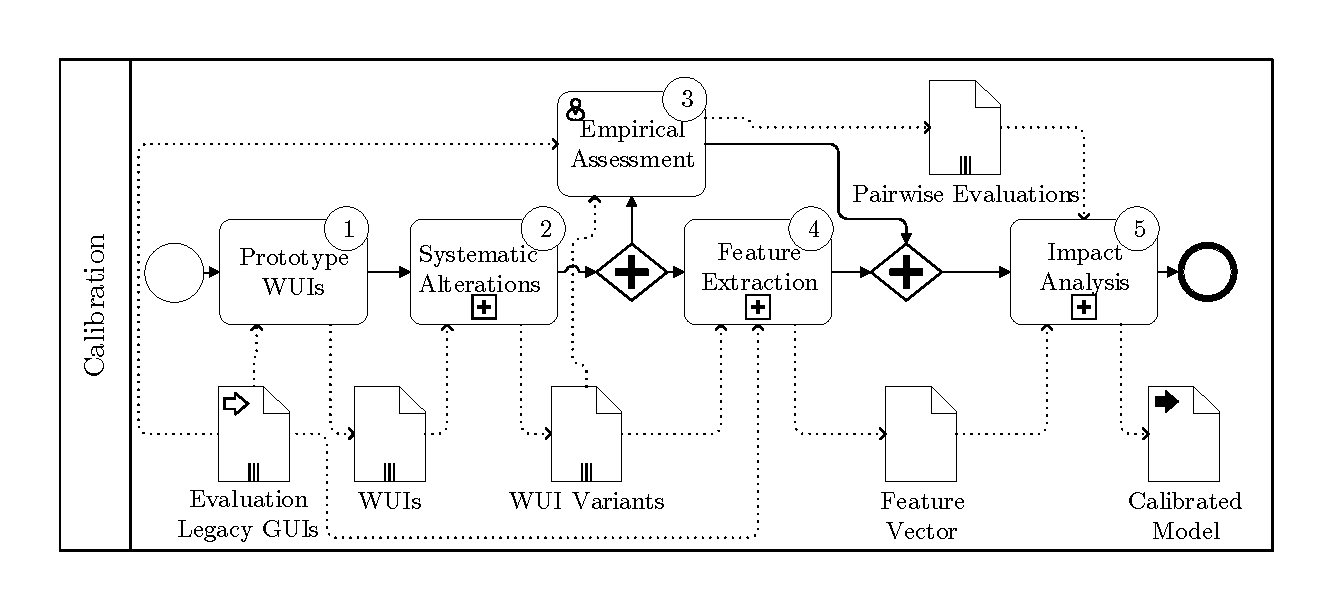
\includegraphics[width=0.99\textwidth]{../figures/awsm-ci-calibration.pdf}
\caption{Calibration Process}\label{fig:ci-calibration}
}
\end{figure}

The calibration process is shown in \cref{fig:ci-calibration}.
It creates \gls{web} user interface prototypes (1) for a set of evaluation \glspl{gui} from the \gls{Legacy System}, e.g.~using the UI \gls{Transformation} technique of AWSM:RM described in \cref{sec:uitransformation}.
Then, these \gls{web} user interfaces are systematically altered with regard to different visual features, similar to the genome mutation strategy in \cref{sec:uitransformation}.
Representatives of the target user group provide pair-wise similarity evaluations for pairs of one \glslink{Legacy System}{legacy} \gls{gui} and one \gls{web} user interface variant through empirical assessment (3).
This step is equivalent to the evaluation of fitness in \cref{sec:uitransformation}.
\Cref{fig:orientation} shows an example of a layout variation, altering the base layout of a patient data input form in \cref{fig:orientation-a} in terms of Orientation, which results in \cref{fig:orientation-b}.
The two highlighted form groups A and B are re-arranged, creating a layout variation with a more pronounced wide-screen aspect ratio, and the aspect ratios of A and B changed in the opposite direction.
Such pairs can be used for the empirical assessment to calibrate the similarity model.
As becomes evident in the example, layout dimensions are not entirely independent: the prominent change in Orientation also influences Density and Order to some extent.

The calibration process uses the same feature extraction (4) like step (4) of the overall Visual UI Similarity Analysis process in \cref{fig:ci-process}, producing a feature vector.
Through combined analysis of the feature vector and the pair-wise evaluations, a \emph{calibrated model} is derived, representing weights according to the impact of features.
This calibrated model can then be used as input model for step (5) in \cref{fig:ci-process}.
The computation of Visual \gls{ui} Similarity described in  \cref{sec:computing-sim} supports this calibration process  through computation of similarity measures with adjustable weights for different perceptual features.

\vspace{-25pt}
\hypertarget{sec:computing-sim}{%
\subsection{Computing Visual UI Similarity}\label{sec:computing-sim}}
\vspace{10pt}

This section describes the implementation of the AWSM:CI method by describing the realization of Visual \gls{ui} Similarity Analysis and Calibration through computation of adjustable similarity measures.
The section provides an answer to the AWSM:CI research question RQ3.

\emph{Similarity measures} play a crucial role in Case-based reasoning (CBR) systems, also known as similarity searching systems.
A similarity measure quantifies the ``degree of resemblance between a pair of cases'' \autocite{Liao1998}.
For AWSM:CI these cases are two versions of a user interface.
To compute the AWSM:CI similarity measure, the \emph{distance-based (computational) approach} is applied, which defines the similarity measure based on a \emph{distance} calculated from objects (features) of the cases (\glspl{ui}).
We define three variations of the \textbf{AWSM:CI similarity measure}: 

\(sim_E\) based on Euclidean distance:
\vspace{-5pt}
\begin{equation}sim_E(\vec x_{u_1}, \vec x_{u_2}) = 1- \text{DIST}_E(\vec x_{u_1}, \vec x_{u_2}) = 1 - \sqrt{\sum\limits_{i=1}^{d} w_i^2 \text{dist}^2(x_{u_1,i}, x_{u_2,i})} \label{eq:sim_e}\end{equation}

\vspace{-10pt}
\(sim_H\) based on Hamming distance:
\vspace{-5pt}
\begin{equation}sim_H(\vec x_{u_1}, \vec x_{u_2}) = 1- \text{DIST}_H(\vec x_{u_1}, \vec x_{u_2}) = 1 - \sum\limits_{i=1}^{d} w_i \text{dist}(x_{u_1,i}, x_{u_2,i})\label{eq:sim_h}\end{equation}

\vspace{-10pt}
and \(sim_R\) based on Tversky ratio mode:
\vspace{-5pt}
\begin{equation}sim_R(\vec x_{u_1}, \vec x_{u_2}) = \frac{\alpha \times \text{common}}{\alpha \times \text{common} + \beta \times \text{different}} \label{eq:sim_r}\end{equation}

for \(\vec x_{u_1}, \vec x_{u_2} \in \mathbb{R}^d; w_i \in \mathbb{R}^+\) and \(\text{common},\text{different} \in \mathbb{N}_0; \alpha, \beta \in \mathbb{R}^+\).

The similarity functions \(sim_E\), \(sim_H\) and \(sim_R\) are similarity \emph{measures} \autocite{ISO/IEEE2017Measurement}, not \emph{metrics}, because a metric requires a \emph{metric space} fulfilling the three axioms of positive definiteness, symmetry, and triangle inequality.
This is not the case for \(sim_E\), \(sim_H\) and \(sim_R\).
However, \(\text{DIST}_E\) and \(\text{DIST}_H\) can be shown to be \emph{pseudo-semimetrics}, i.e.~fulfilling positivity, symmetry, and the relaxed positive definiteness axiom as one-sided implication \(\vec x = \vec y \implies \text{DIST}_E(\vec x, \vec y) = \text{DIST}_H(\vec x, \vec y) = 0\).

\begin{figure}[h!]
\centering

\subfloat[Layout]{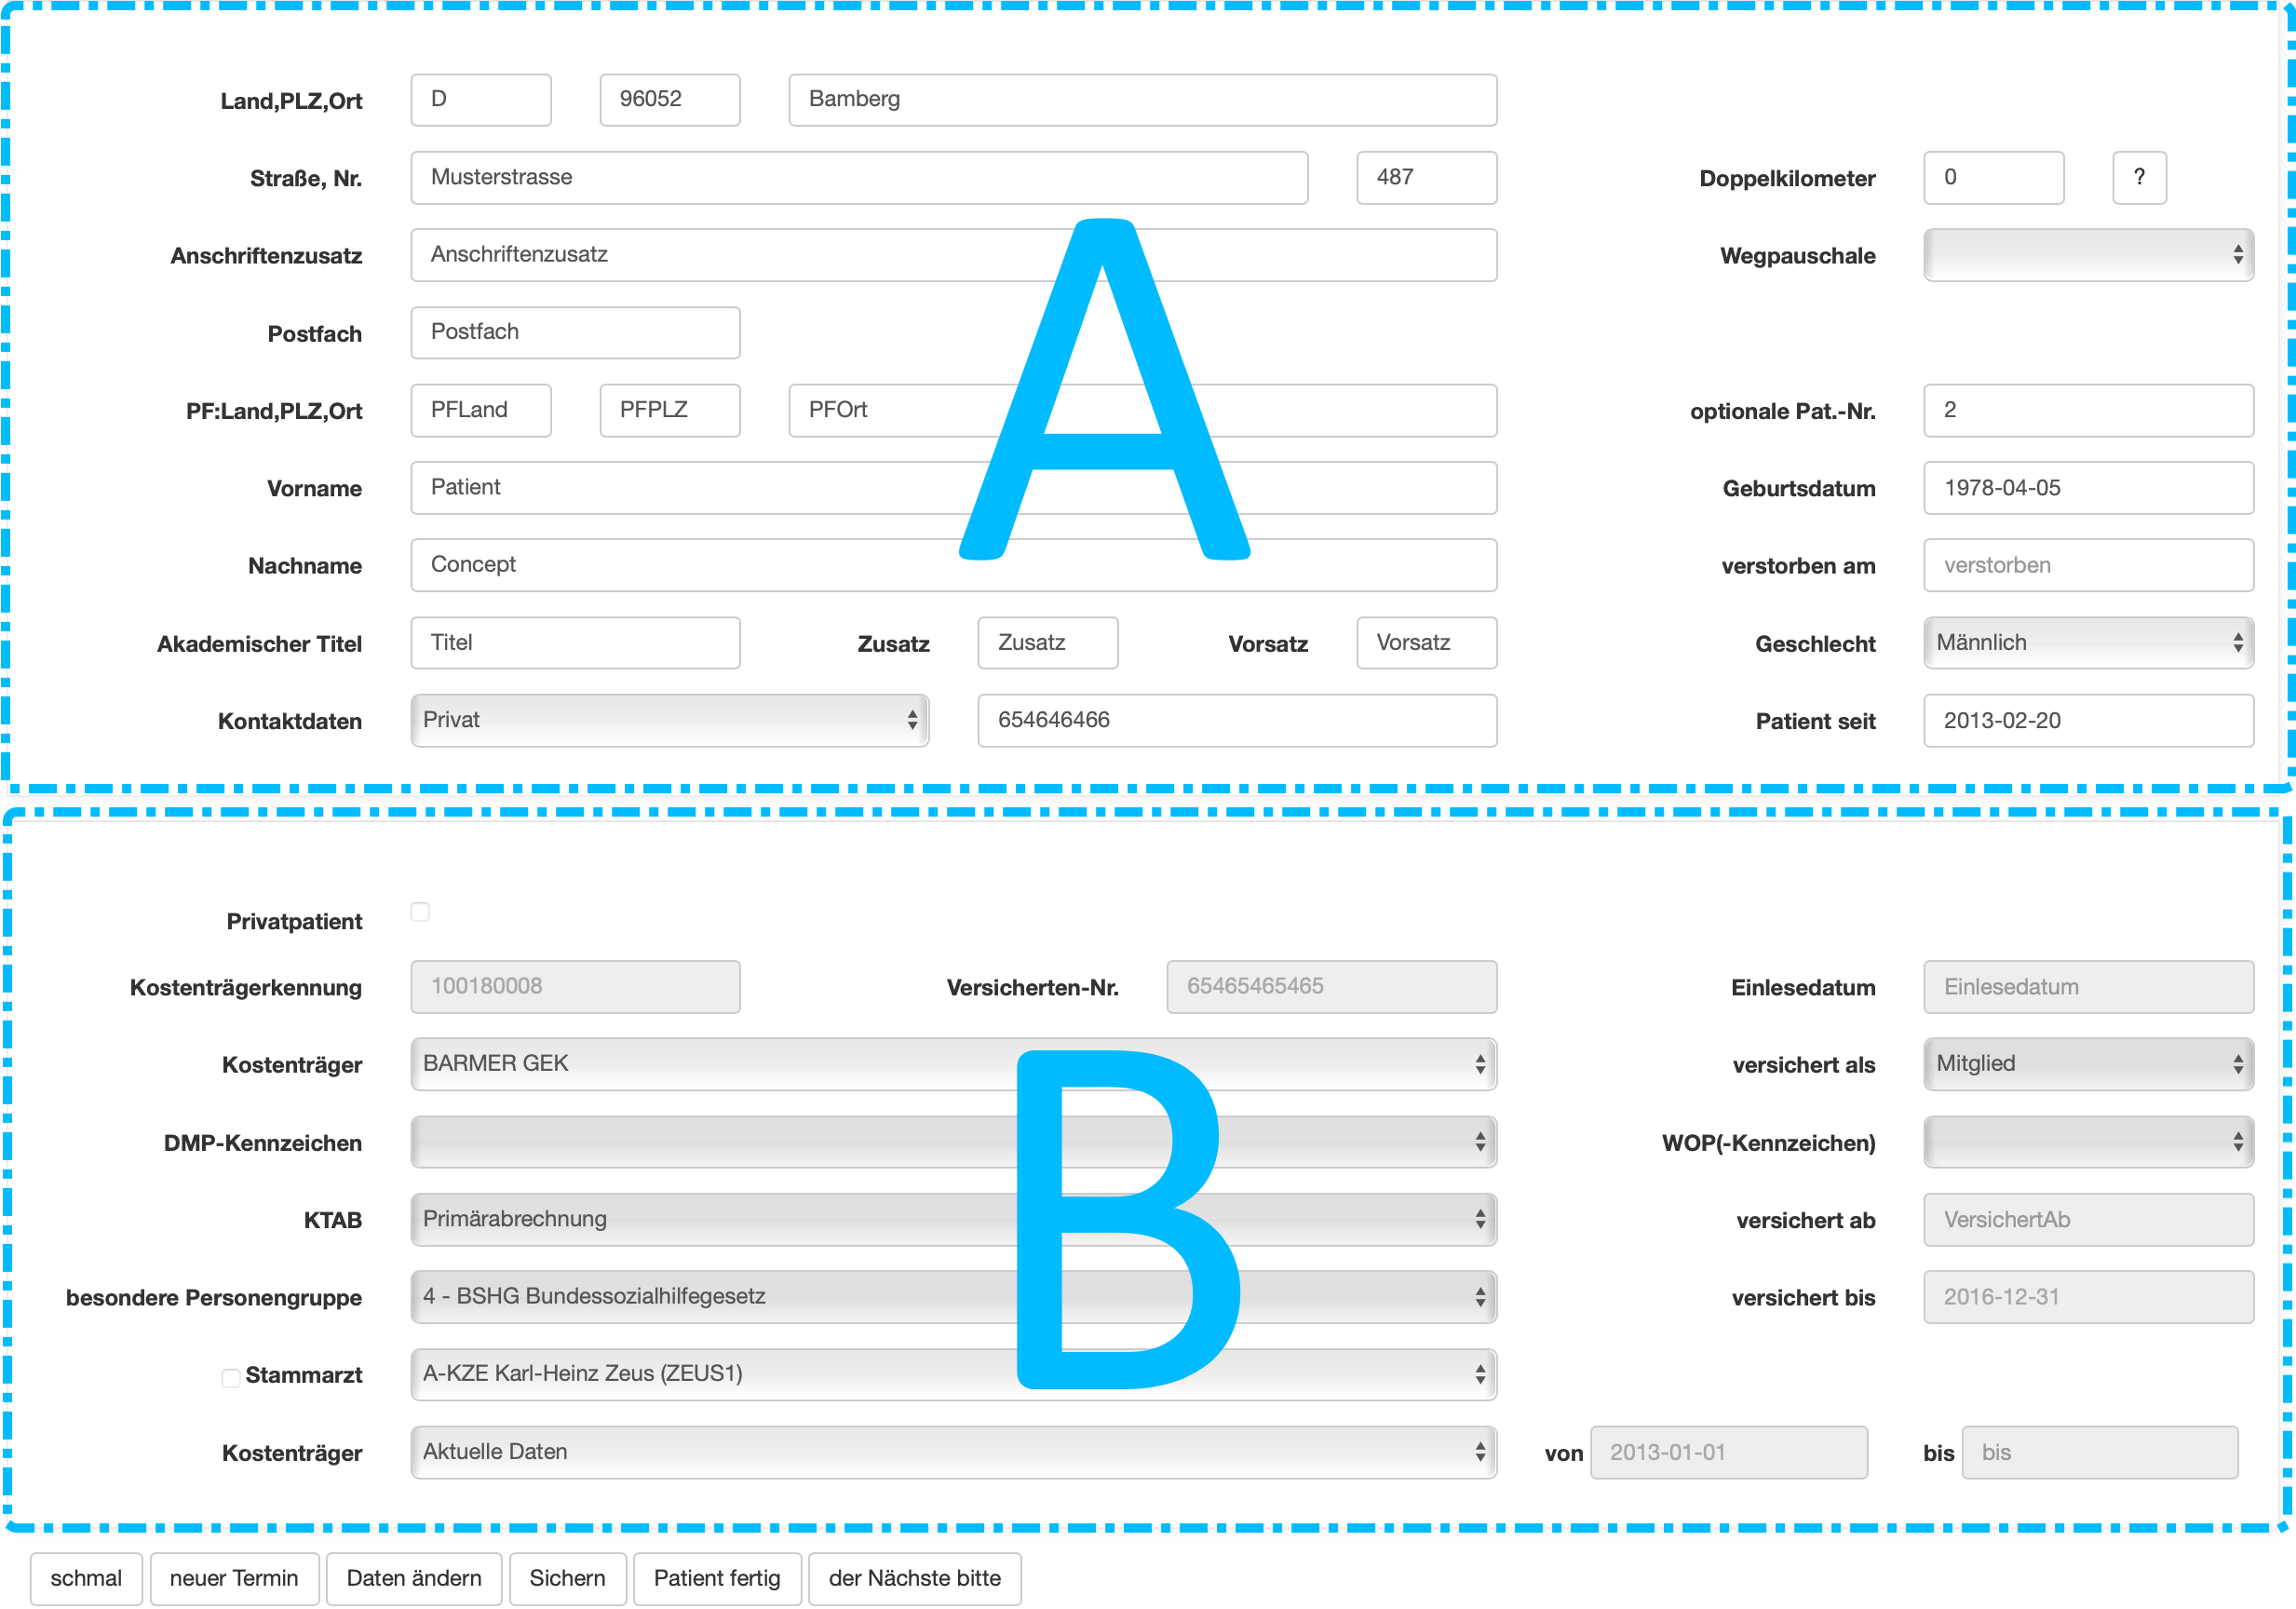
\includegraphics[width=0.85\textwidth]{../figures/screenshots/orientation1-new-overlay.png}\label{fig:orientation-a}}

\subfloat[Orientation Variation]{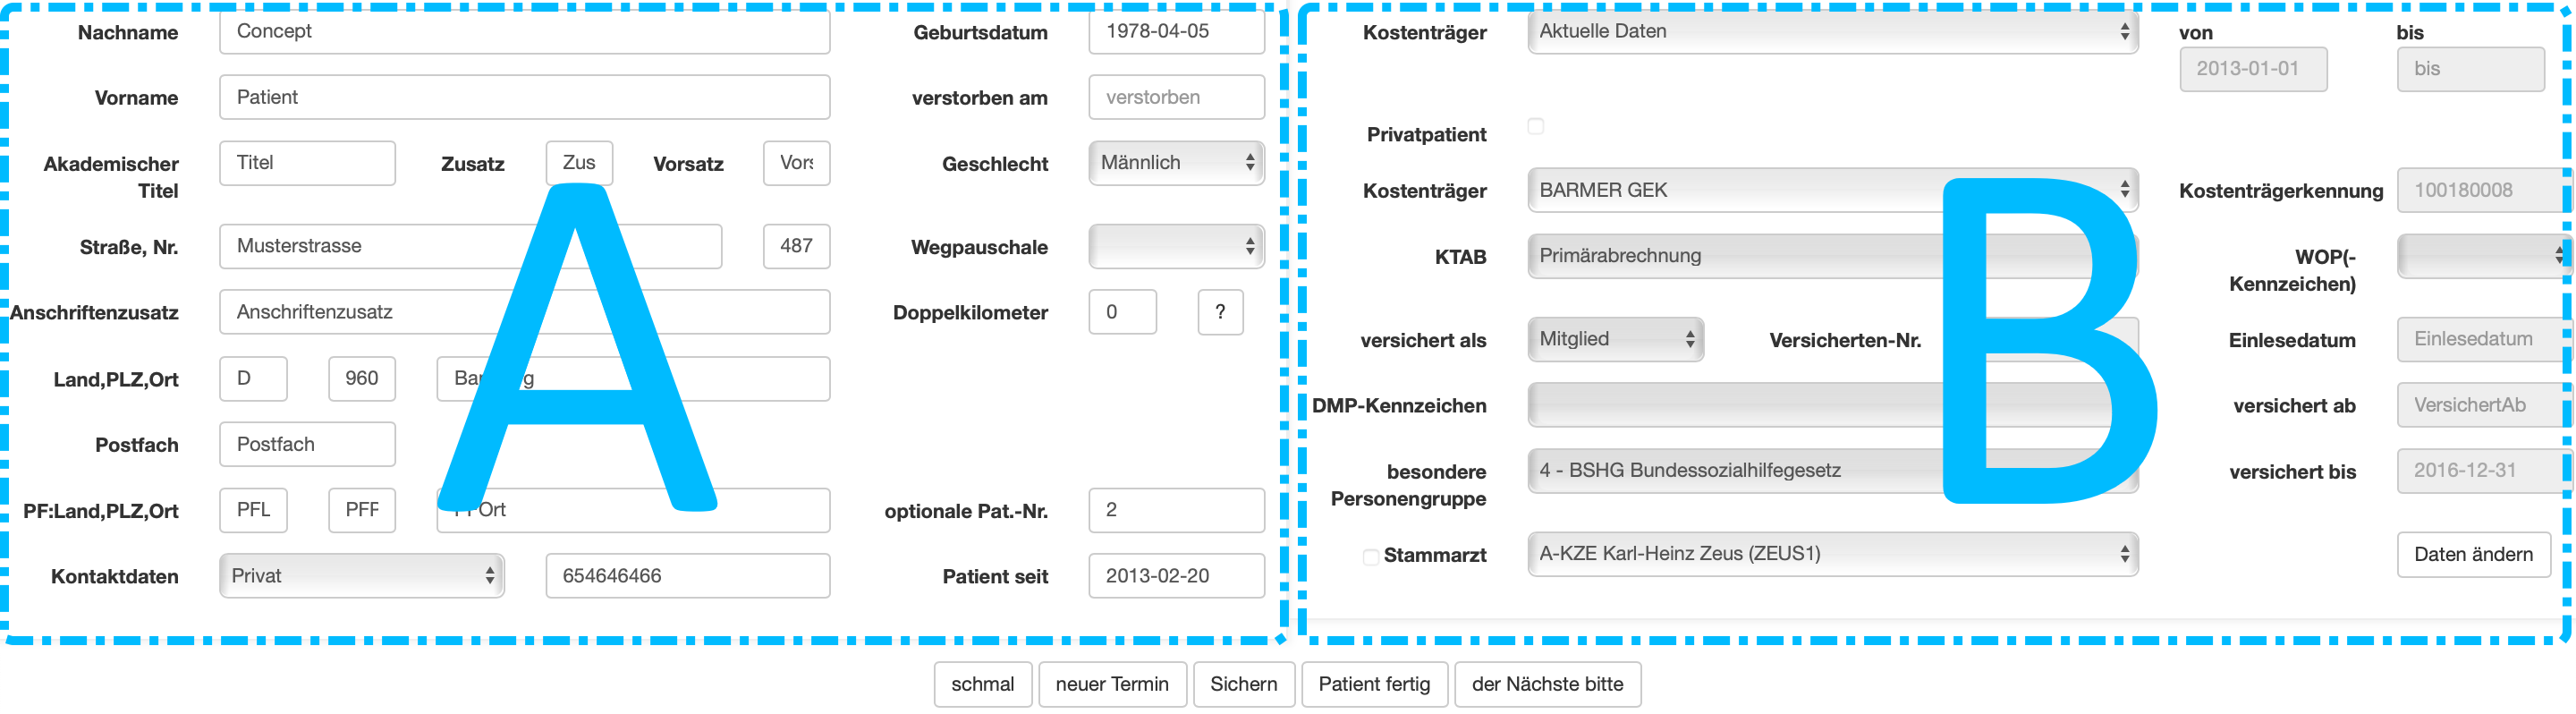
\includegraphics[width=0.95\textwidth]{../figures/screenshots/orientation2-new-overlay.png}\label{fig:orientation-b}}

\caption{Layout Variations}

\label{fig:orientation}

\end{figure}

\emph{Feature-based normalized distance functions} \(\text{dist}\) define the calculation of \(\text{DIST}_E\) and \(\text{DIST}_H\), and the weight factors \(w_i\) allow for the calibration process in \cref{sec:calibration} to adjust the impact of different features.
AWSM:CI uses three distances in the Layout dimension of \gls{ui} Similarity: Orientation, Order, and Density \autocite{Heil2016Similarity}.
\Cref{fig:ci-dimensions} illustrates these three aspects for distance calculation.
When migrating a \legacy layout like in the top left, orientation changes can result from different available screen sizes, as shown in the top right.
Order of elements or container elements can change due to the distribution into rows and columns, causing some elements to be assigned to a new row, as shown in the bottom left.
Density can change due to different element sizes caused by changes in the Material dimension, i.e. different visual appearance and resulting size of controls like buttons, as shown in the bottom right.
As seen, changes in one aspect may also produce changes in other aspects.

\begin{figure}[h!]
\hypertarget{fig:ci-dimensions}{%
\centering
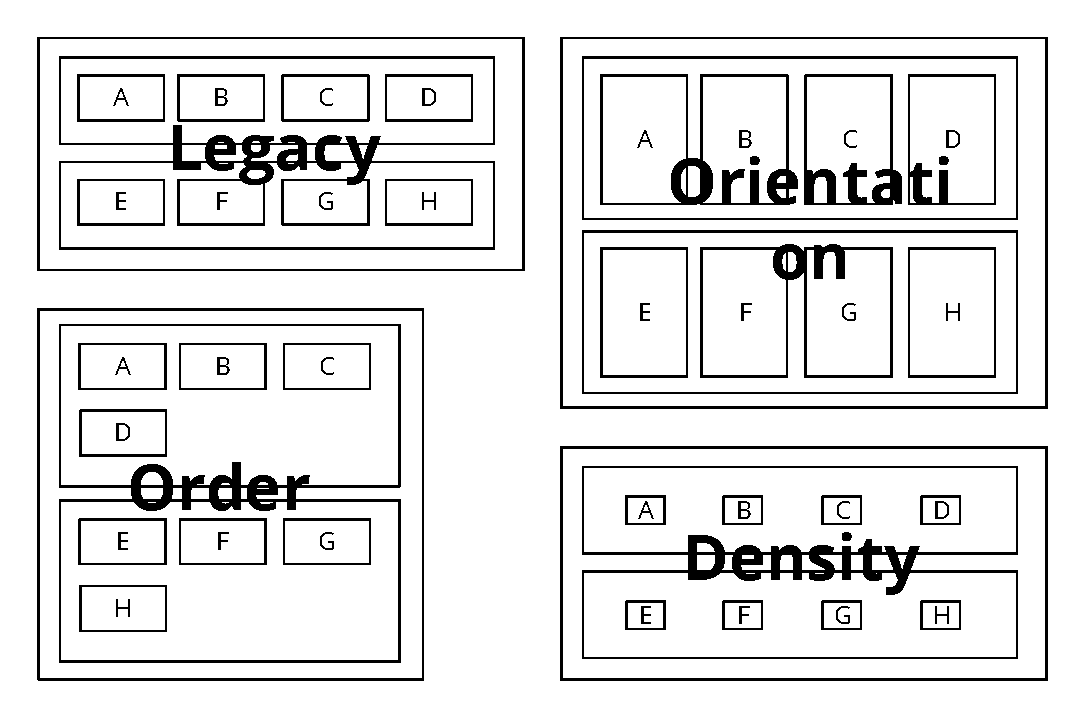
\includegraphics[width=0.75\textwidth]{../figures/awsm-ci-similarity-dimensions.pdf}
\caption[Orientation, Order and Density Changes]{Legacy Layout and Changes in Orientation, Order and Density }\label{fig:ci-dimensions}
}
\end{figure}

All three distances are normalized to percentages using Tversky difference ratios with \(\alpha = \beta = 1\):
\begin{equation}\text{dist}(x_{u_1,i}, x_{u_2,i}) = \frac{\text{different}}{\text{different} + \text{common}}\label{eq:dist}\end{equation}

These distances represent \emph{base measures} \autocite{ISO/IEEE2017Measurement} and are computed on the four different levels of the \gls{ui} hierarchy introduced in \cref{sec:segmentation}, region, block, group, and atomic elements.
For \emph{Orientation}, this results in the share of \glspl{roi} that have a different visual orientation.
These orientations can be one of \(\{\text{vertical}, \text{horizontal}, \text{other}\}\).
Vertical orientation represents aspect ratios of bounding box \(b\) (cf.~\cref{eq:bounding-box}) with \(w/h < \theta_O\) (i.e.~portrait), horizontal orientation represents aspect ratios of \(w/h > 1 / \theta_O\) (i.e.~landscape), other orientation implies \(w/h \approx 1\) (i.e.~approximate square).
These can be calculated from a pair-wise comparison of the bounding boxes using threshold parameter \(\theta_O\in\mathbb{R}, 0<\theta_O < 1\).
Assignment to class \(\text{different}\) or \(\text{common}\) is based on equality comparison of the resulting nominal orientation variable.
\Cref{fig:orientation} shows an example of a \gls{wui} created for the scenario application described in \cref{sec:scenario} and a layout variation with different orientation.
\emph{Order} differences can be computed using Levenshtein distances in 8 different orientations (left to right top to bottom, bottom to top right to left, etc.) on sequences, as described in \cref{sec:uitransformation.tool}.
Assignment to class \(\text{different}\) is equivalent to a Levenshtein distance of \(\text{dist}_L > 0\), else \(\text{common}\) is assigned.
\emph{Density} represents the share of \glspl{roi} with different visual density.
Computation of Density is based on bounding boxes, calculating the white space ratio \(W\) \autocite{Bakaev2019JWE}, i.e.~the ratio of the area occupied by nested \glspl{roi} to the overall area.
Assignment to class \(\text{common}\) is based on threshold parameter \(\theta_D\in\mathbb{R}, 0<\theta_D < 1\) if and only if \(W_1/W_2 \in [ \theta_D, 1/\theta_D]\).
The distances are specific for \gls{Web Migration} as they require the two compared user interfaces \(u_1\) and \(u_2\) to share a significant common subset of \gls{ui} Elements: \(\frac{|E_{u_1} \cap E_{u_2}|}{|E_{u_1} \cup E_{u_2}|} > 1 - \varepsilon\).

%\pagebreak
\hypertarget{sec:ci.integration}{%
\subsection{Integration with Ongoing Development}\label{sec:ci.integration}}
\vspace{10pt}

As described in \cref{g:1}, the neglect of integration with ongoing agile software development activities (\cref{c:4} Agile) limits the applicability of many \gls{Web Migration} approaches.
Therefore, the AWSM:CI method needs to be integrated with ongoing daily development activities of the \gls{isv}.
\Cref{fig:ci-process} specifies a measurement-based process to be used during the \gls{Forward Engineering} phase, i.e.~the creation of the \gls{target system}, of a \gls{Web Migration}, corresponding to a \emph{design measurement} of the implementation phase of software maintenance \autocite{IEEE1219Maintenance}.
Thus, its integration into ongoing forward development activities can be easily achieved.
The measurement is based on automatic computer vision-based analysis and computation of similarity measures and does not require manual interaction apart from triggering the measurement.
The measurement activity should be repeatedly triggered during the creation of \gls{web} versions of user interfaces to guide design decisions.
The integration point can be parallel to other software quality measurements like cyclomatic complexity or function points \autocite{Kan1996Metrics} for both model-driven and non-model-driven development processes (cf.~principle \cref{p:3}).
If no dedicated measurement activities are specified in the ongoing development model, integration of AWSM:CI has to be achieved in an ad-hoc manner into user interface design activities following the \gls{ieee} recommendations on performing measurement processes \autocite{SWEBOK2014}.
While the measurement process itself can be started by any \gls{migrationengineer}, the calibration process  should be executed by staff with expertise in empirical methods.
For an \gls{isv} as in \cref{sec:company-characteristics}, the usability experts and \gls{uix} designers, forming a dedicated team called Team U in medatixx, are well-suited due to their understanding of user interaction and qualification for empirical user analysis.
Thus, when dedicated \gls{uix} experts are available in the \gls{isv}, integration of AWSM:CI can be achieved in the context of the ongoing \gls{Forward Engineering} \gls{uix} analysis and approval activities.
On \glspl{artifact} level, the similarity measures represent another software quality measurement, if measurement activities are present, and are to be integrated into the corresponding set of measurement \glspl{artifact}.
If no measurement activities are present, the similarity measures represent a new type of software \gls{artifact} which should be integrated into configuration management and expressed using an open standard (cf.~principle \cref{p:1}) such as \gls{smm} \autocite{OMG2012SMM} or the \gls{ieee} measurement information model \autocite{ISO/IEEE2017Measurement} to allow for interoperability.

\vspace{-10pt}
\hypertarget{sec:segmentation}{%
\section{Visual UI Element Detection}\label{sec:segmentation}}
\vspace{20pt}

To conduct the Visual UI Similarity Analysis described in \cref{sec:visual-analysis} with limited resources according to \cref{ro:3}, this section describes a technique Visual UI Element Detection.
Computation of the similarity function \(sim\) is based on distances in \gls{ui} layouts.
Most of these distances are depending on \gls{ui} Elements:
Distance in Orientation is calculated from aspect ratios of bounding boxes of high-level container \gls{ui} Elements.
Order distances compare positions of \gls{ui} Elements on the viewport.
Distance in Density uses Whitespace Ratio, which requires distinguishing areas occupied by \gls{ui} Elements from areas that are empty.
While \gls{ui} Elements can be easily identified by human actors for whom graphical user interfaces are designed, this manual detection would be a very time-consuming activity that has to be repeated many times when using AWSM:CI, violating the limited resources constraint of \cref{ro:3}.
Therefore, the technical challenge that needs to be addressed lies in the automation of Visual \gls{ui} Element Detection as defined by steps (2) and (3) of \cref{fig:ci-process}, providing the second part of the answer to AWSM:CI RQ3.
\Cref{sec:segmentation.concept} outlines the conceptual model for Visual \gls{ui} Element Detection, and \cref{sec:segmentation.impl} describes the implementation in the Visual UI Element Detector Tool of the \gls{awsm} Toolsuite.

\vspace{-15pt}
\hypertarget{sec:segmentation.concept}{%
\subsection{Conceptual Model}\label{sec:segmentation.concept}}
This section defines the conceptual model of Visual \gls{ui} Element Detection in AWSM:CI by identifying the three involved perspectives on user interfaces and defining the related concepts and relationships, as presented in \cref{fig:ci-concepts}.
\begin{figure}[h!]
\hypertarget{fig:ci-concepts}{%
\centering
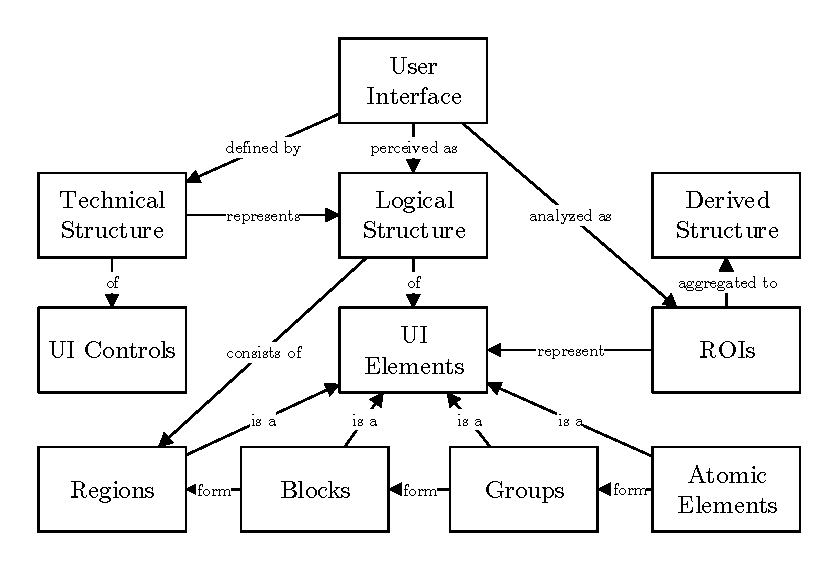
\includegraphics[width=0.75\textwidth]{../figures/awsm-ci-concepts.pdf}
\caption{User Interface Concept Map}\label{fig:ci-concepts}
}
\end{figure}

By extending the user interface formalism in \cref{sec:ui-formalism}, this conceptual model allows for a visual bottom-up \gls{Reverse Engineering} process of the user interface that works across \glslink{Legacy System}{legacy} and \gls{web} platforms, addressing the applicability requirement in \cref{sec:ci.requirements}.
As it focuses on the identification of \glspl{roi} and deriving the structure through computer vision techniques instead of parsing the technical structure, the segmentation is independent of specific \gls{gui} technologies.

The user interface formalism in \cref{sec:ui-formalism} introduced the concept of user interfaces \(u\) being composed by a set of \gls{ui} controls \(C_u\), with controls \(c\in C_u\) forming a hierarchy through parent-child relationships.
These controls represent the \emph{technical perspective} on a user interface \(u\) and are derived from their descriptions (\gls{kdm} SourceFiles, ConfigFiles, Documents) in codebase \(B\).
To represent the \emph{visual perception perspective}, \emph{\gls{ui} Elements} are introduced.
\gls{ui} Elements are the constituents of \(u\) visually perceived by human users forming its \emph{logical/semantic structure}.
There is no direct mapping between \gls{ui} Controls and \gls{ui} Elements: a \gls{ui} Control may not be visually perceived as \gls{ui} Element, and one \gls{ui} Element may be composed of several \gls{ui} Controls.

\gls{ui} Elements form a similar hierarchical structure like \gls{ui} Controls defined through spatial relationships like containment, alignment, and proximity.
To represent aspects of \emph{visual complexity} \autocite{Bakaev2019JWE} in this hierarchy, which is known to have significant influence on perception \autocite{Tuch2009VisualComplexity}, we introduced four distinct levels of \gls{ui} Elements: Regions, Blocks, Groups and atomic Elements \autocite{Heil2016Similarity}.
\emph{Atomic Elements} \autocite{Bakaev2019JWE} are \gls{ui} Elements without nested \gls{ui} Sub-Elements; examples are buttons, inputs, or checkboxes.
Through alignment and proximity, they form \emph{Groups} like vertically aligned labels in a form.
\emph{Blocks} are formed from Groups and typically represent domain entities, e.g.~entire forms.
\emph{Regions} are formed from Blocks and represent the top-level visual structure of a page such as navigation, header, content area.

To automate visual analysis, automatic recognition of \gls{ui} Elements is required.
This introduces the third perspective on a \gls{ui}: the \emph{recognition perspective}, which represents the perspective of a technical solution to approximate the visual perception perspective.
Visual \gls{ui} Element Detection tries to simulate human understanding of a user interface through the identification of its constituents based on visual aspects.
This consists of two tasks: identification of Regions of Interest and classification of the type of these \glspl{roi}.
Thus, \glspl{roi} are the recognition perspective concept on a similar level, like \gls{ui} Control and \gls{ui} Element.
However, the completeness and correctness of the mapping between \gls{ui} Elements and \glspl{roi} depend on the quality of the \gls{gui} Segmentation.
Also, \glspl{roi} can be smaller than Atomic Elements, e.g.~the text label on a button is an \gls{roi} detectable through \gls{ocr}.

\vspace{-10pt}
\hypertarget{sec:segmentation.impl}{%
\subsection{Visual UI Element Detector}\label{sec:segmentation.impl}}
\vspace{10pt}

This section describes the implementation of the Visual \gls{ui} Element Detection subprocess in \cref{fig:ci-process}.
Visual \gls{ui} Element Detection consists of locating and classifying \gls{ui} Elements in screenshots of \legacy desktop or \web user interfaces.
Thus, the process of Visual \gls{ui} Element Detection shown in \cref{fig:ci-vued} is split into two parts: location of \glspl{roi} and classification.
Detection of \gls{ui} Elements is object detection with specific features that distinguish it from other application domains: absence of image phenomena appearing in photos such as noise, glare, uneven lighting, perspective distortion, movement, incomplete or covered objects make analysis easier \autocite{Bakaev2019JWE}.
On the other hand, \gls{ui} Elements are relatively small (e.g.~a checkbox) objects, have very similar, non-distinctive shapes (e.g.~buttons and input fields), have different stateful visual appearances (e.g.~checked and unchecked radio buttons), have different appearances in different platforms (e.g.~buttons in MacOS vs.~Windows), can occur on top of background images without differences in lighting or focus helping to distinguish layers, and have composite nature requiring context (e.g.~checkbox and its label, a group of tabs), which makes \gls{ui} Element Detection difficult.
A \emph{sound} and \emph{complete} (i.e.~high precision and maximum recall) mapping of \gls{ui} Elements in two \glspl{ui} based on computer vision is an \emph{undecidable problem} \autocite{Grechanik2018}.

\begin{figure}[h!]
\hypertarget{fig:ci-vued}{%
\centering
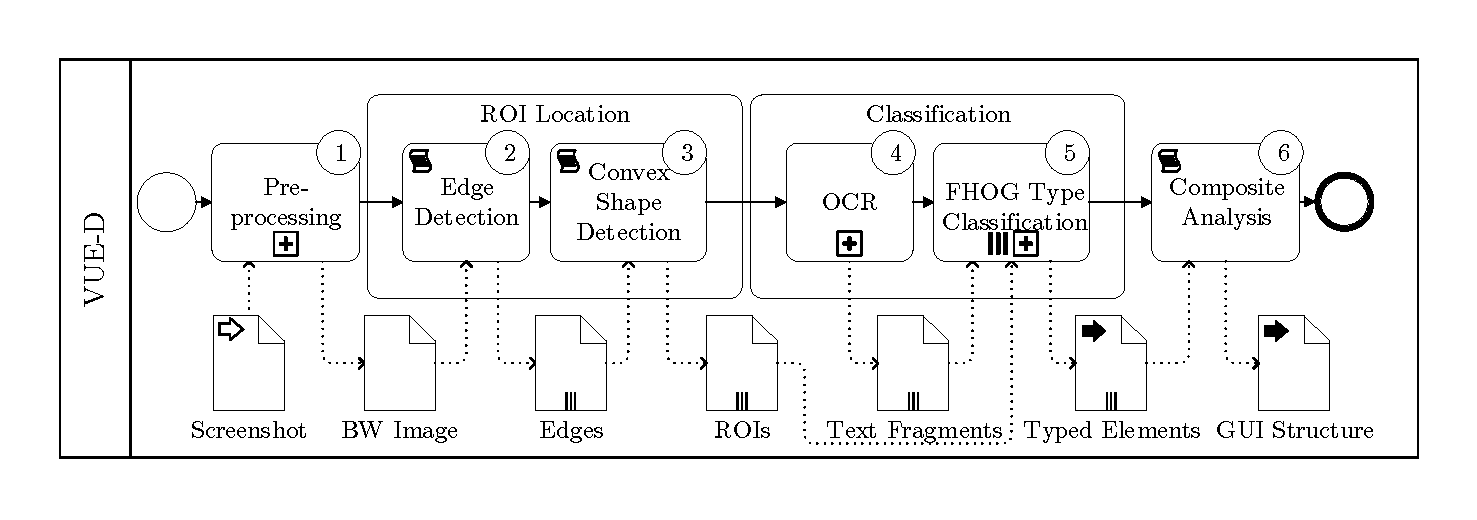
\includegraphics[width=0.99\textwidth]{../figures/awsm-ci-vued.pdf}
\caption{VUE-D Analysis Process}\label{fig:ci-vued}
}
\end{figure}

The \emph{\gls{vued}} is implemented based on the computer vision strategy by \citet{Kong2012} as part of the \gls{hci} Vision approach \autocite{Bakaev2019JWE,Bakaev2018ICWE} and is embedded in the \gls{ui} Metrics integration platform\footnote{\url{http://va.wuikb.info/} Retrieved: 8.12.2019} \autocite{Bakaev2019ICWE}.
\Cref{fig:ci-vued} shows the \gls{vued} analysis process.
The \gls{ui} screenshot is subject to \emph{preprocessing} (1) to improve detection results.
It consists of grayscale conversion, upscaling, and black-and-white conversion using thresholding.
OpenCV\footnote{\url{https://opencv.org/} Retrieved: 6.12.2019} is used for these tasks.
\emph{Detection of \glspl{roi}} is implemented using OpenCV's edge detection (2) for vertical and horizontal lines in the binary image.
The rectangles are identified from edges as convex shapes (3) with 4 corners of a minimum area as boxes \(b\), according to \cref{eq:bounding-box}.
For \emph{\gls{ocr}} (4), \gls{vued} combines OpenCV close edge detection with \emph{Tesseract}\footnote{\url{https://github.com/tesseract-ocr/tesseract} Retrieved: 6.12.2019}.
It identifies areas of high-frequency edges, does upscaling, and then performs \gls{ocr} using Tesseract.
For successful recognitions, the results are represented as bounding boxes \(b\), and the recognized text is annotated as additional information.
The \emph{type classification} (5) uses specialized classifiers for different types of \gls{ui} Elements.
Each classifier is trained on one specific type using supervised learning on the \gls{fhog} latent SVM feature \autocite{Felzenszwalb2010FHOG} extractor implemented in dlib\footnote{\url{http://dlib.net/} Retrieved: 6.12.2019} which represents each input as 31-dimensional \gls{fhog} feature vector.
Due to high visual differences, stateful elements like checkboxes, radio buttons are trained separately, as are platform variations.
The classification result is then annotated as additional information to the \gls{roi}.
\emph{Composite Analysis} (6) identifies composite \gls{ui} Elements using alignment, proximity, and containment, for instance combining recognized text labels with checkboxes, etc.
by merging their bounding boxes.
The architecture of VUE-D is shown in \cref{fig:ci-vued-architecture}.
\Cref{fig:ui-recognition} shows application of \gls{vued} on a screenshot of the \gls{gui} from \cref{fig:orientation-b} with detection results highlighted.
\begin{figure}[hbt]
\hypertarget{fig:ui-recognition}{%
\centering
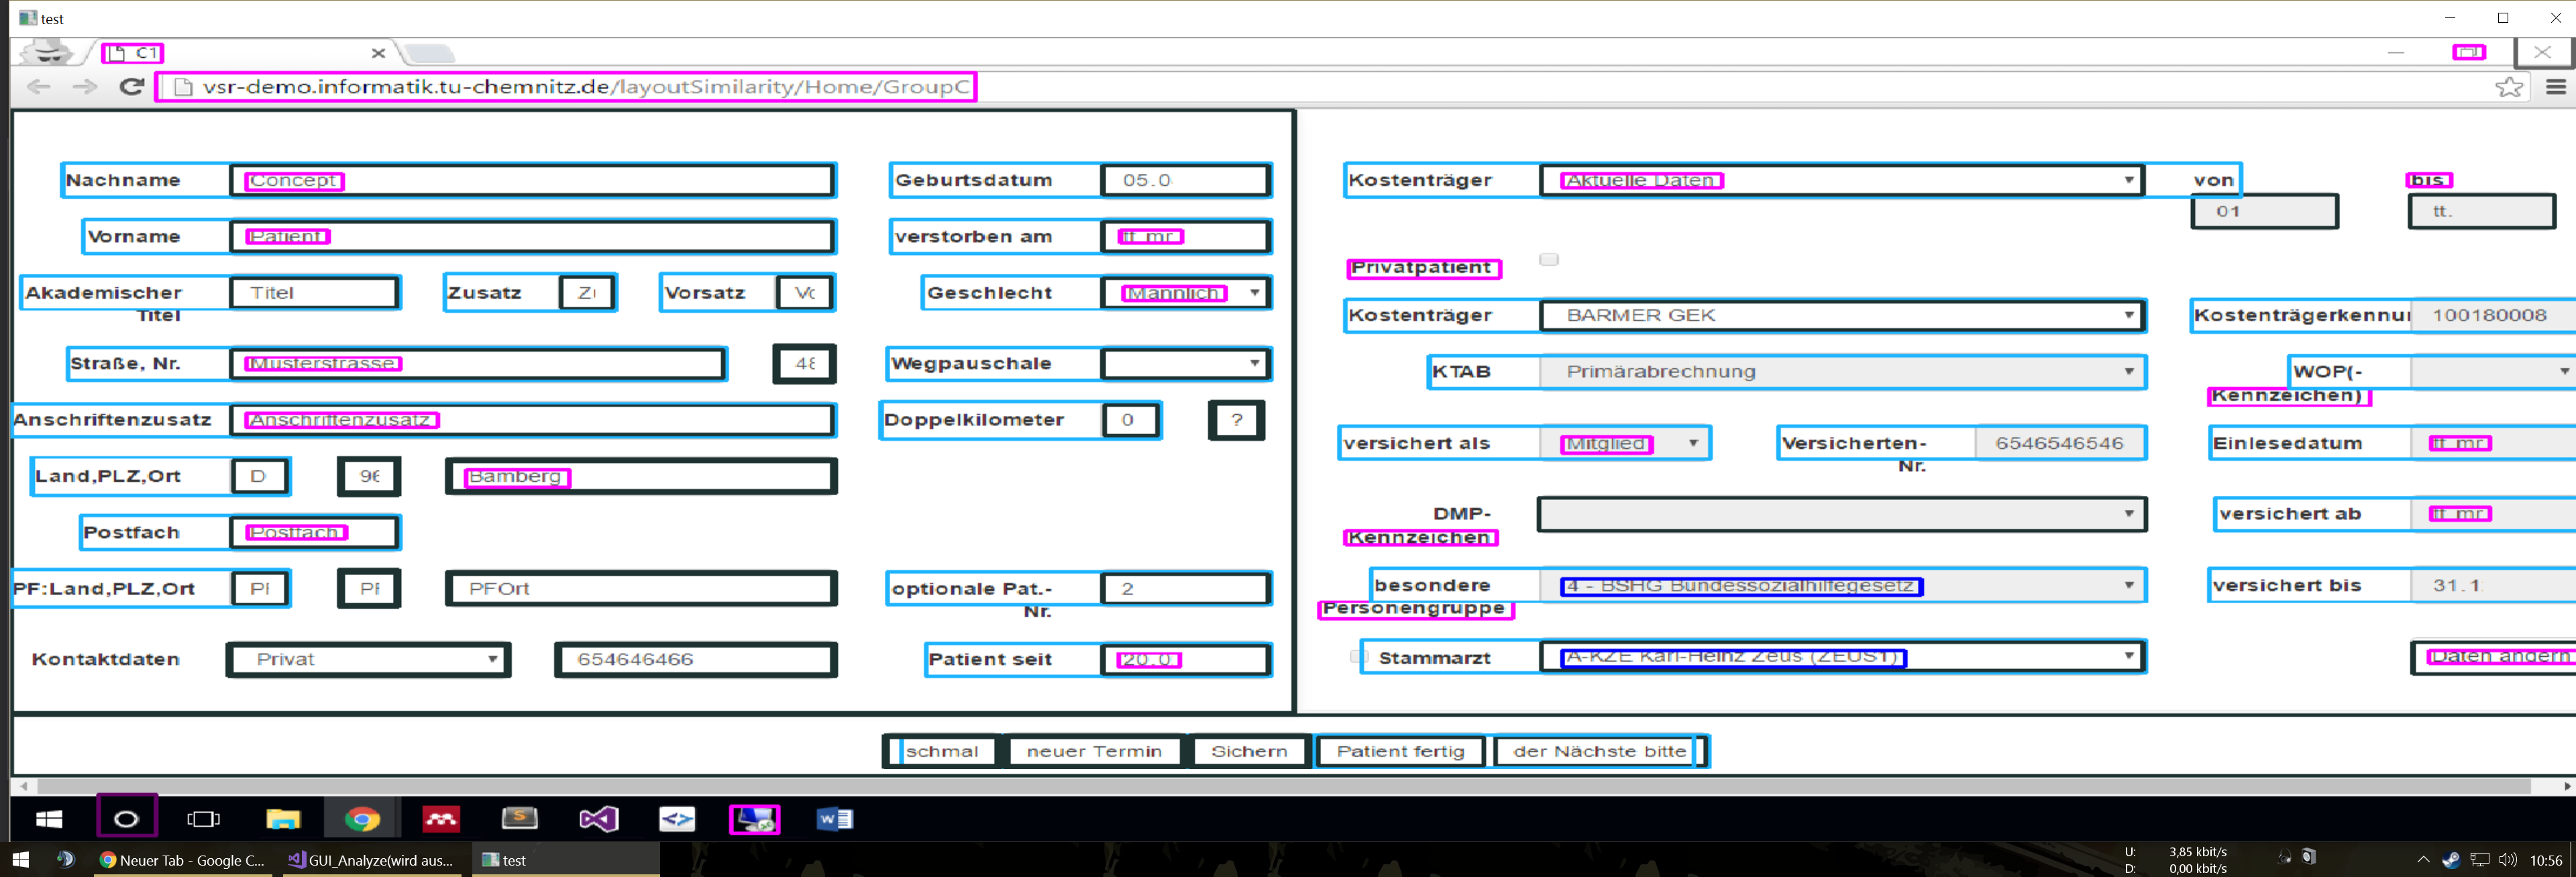
\includegraphics[width=0.99\textwidth]{../figures/segmented-wui.png}
\caption[Visually Segmented Screenshot from VUE-D]{Visually Segmented Screenshot from VUE-D, pink highlights show OCR results, black hightlights indicate indicate convex shape detection results, blue highlights indicate composites}\label{fig:ui-recognition}
}
\end{figure}
\begin{figure}[h]
\hypertarget{fig:ci-vued-architecture}{%
\centering
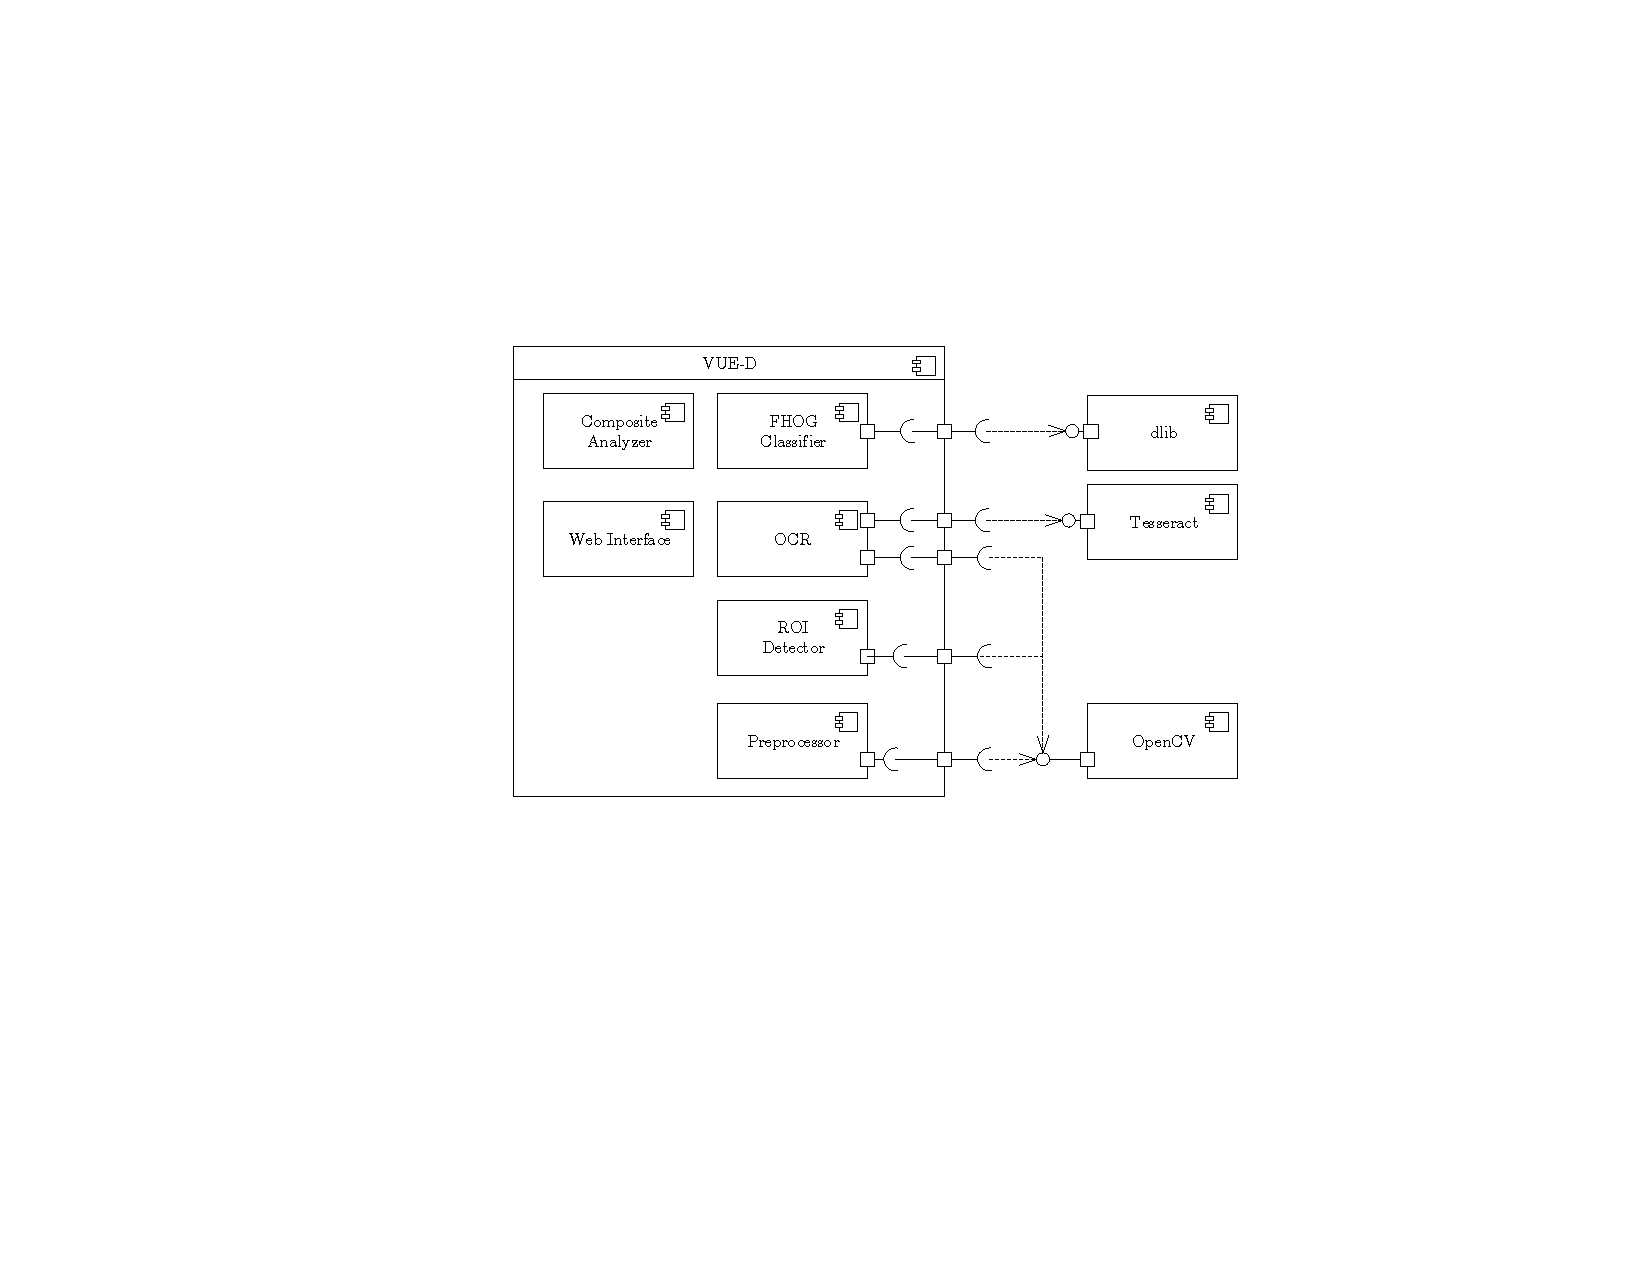
\includegraphics[width=0.99\textwidth]{../figures/awsm-ci-vued-architecture.pdf}
\caption{VUE-D Architecture}\label{fig:ci-vued-architecture}
}
\end{figure}

The \gls{ui} Elements detected by VUE-D are represented using the XML metamodel employed in the Pascal VOC Challenge datasets\footnote{\url{http://host.robots.ox.ac.uk/pascal/VOC/index.html} Retrieved: 6.12.2019}, a de-facto standard for representation of Object Detection results, providing access to an existing environment of viewers, editors and libraries.
\Cref{lst:pascalvoc} shows a shortened example of VUE-D results serialized as Pascal VOC XML.
The sample indicates the screenshot file that was analyzed, the size of the viewport, and it contains three detected objects: a text field, a checkbox, and a button, together with their bounding boxes.

\begin{lstlisting}[language=xml, captionpos=t, caption=VUE-D Detection Results (shortened) represented as Pascal VOC model, label=lst:pascalvoc]
<annotation>
  <folder>test-set</folder>
  <filename>1001.jpg</filename>
  <path>/Users/sebastian/test-set/1001.jpg</path>
  <size>
    <width>2880</width>
    <height>1628</height>
    <depth>3</depth>
  </size>
  <object>
    <name>input_text</name>
    <bndbox>
      <xmin>644</xmin>
      <ymin>65</ymin>
      <xmax>816</xmax>
      <ymax>127</ymax>
    </bndbox>
  </object>
  <object>
      <name>checkbox</name>
      <bndbox>
        <xmin>462</xmin>
        <ymin>1295</ymin>
        <xmax>489</xmax>
        <ymax>1328</ymax>
      </bndbox>
    </object>
    <object>
      <name>button</name>
      <bndbox>
        <xmin>237</xmin>
        <ymin>1469</ymin>
        <xmax>357</xmax>
        <ymax>1531</ymax>
      </bndbox>
    </object>
</annotation>
\end{lstlisting}

\vspace{-15pt}
\hypertarget{sec:ci.evaluation}{%
\section{Evaluation}\label{sec:ci.evaluation}}
\vspace{15pt}

This section evaluates AWSM:RM regarding three aspects.
\Cref{sec:ci.evaluation.req} evaluates AWSM:CI regarding the requirements in \cref{sec:ci.requirements}.
Additional experimental evaluation further address effectiveness, applicability, and calibratability in \cref{sec:ci.experiment}.
\Cref{sec:ci.evaluation.objective} revisits research objective \cref{ro:3} in the light of the evaluation results.

\vspace{-20pt}
\hypertarget{sec:ci.evaluation.req}{%
\subsection{Assessment of Requirements}\label{sec:ci.evaluation.req}}
\vspace{10pt}

This section reports on satisfaction of the requirements for AWSM:CI.

\textbf{Effectiveness}. The effectiveness of AWSM:CI is achieved through specification of a \gls{ui} Similarity between \glslink{Legacy System}{legacy} and \gls{web} user interfaces that produces concrete measurements to assess different versions of user interfaces, which can be used as a basis for decision making when comparing design alternatives.
A detailed analysis of measurement results is presented in the following evaluation experiment.

\textbf{Efficiency}. Measurement of \gls{ui} Similarity should be supported by analysis tools to automate the measurement process.
The efficiency of AWSM:RM is supported through specification of similarity measures that can be computed based on automatically derived distances.
The computer-vision-based approach for \gls{ui} Element Detection of \glslink{Legacy System}{legacy} and \gls{web} user interfaces is automated but does not yet produce results with production-grade quality.
Thus, the efficiency requirement is considered only half-fulfilled.

\textbf{Expertise}. The computation of similarity measures and the calibration process of AWSM:CI do not require specific expertise and can be conducted using the artifacts (questionnaire) and analysis strategy (factor impact analysis and corresponding model calibration) presented in the following experimental evaluation as a blueprint by any \gls{isv} staff member with reasonable expertise in basic statistics.
Likewise, the test subjects do not have any specific expertise requirements, as the similarity evaluation can be performed by any non-expert target group representative with normal vision.
Thus, the Expertise requirement is considered as satisfied.

\textbf{Applicability}. The AWSM:CI method follows a pure computer vision strategy and does not rely on any specific technology-related analysis.
Instead, the proposed distances and similarity measures can be computed on any image representation of a user interface, both conceptual and implemented, as they consider solely visual aspects of the user interfaces.
Therefore, the Applicability requirement is satisfied.

\textbf{Calibratability}. The AWSIM:CI similarity measures can be calibrated to the perceptual characteristics of the target group following the calibration process described in \cref{sec:calibration}.
The following experimental evaluation shows in more detail how the calibration process can be used to align the similarity measures with empirical evaluation results gathered from a small group of representatives.
The Calibratability requirement is satisfied.

\vspace{-10pt}
\hypertarget{sec:ci.experiment}{%
\subsection{Experimental Evaluation of AWSM:CI}\label{sec:ci.experiment}}
\vspace{10pt}

Experimental evaluation of AWSM:CI demonstrates the application of the similarity computation and calibration process based on a dataset of user interfaces from the real-world scenario application \emph{x.concept} (cf.~\cref{sec:scenario}) with empirical assessments of perceived similarity by test subjects \autocite{Heil2016Similarity}.

\textbf{Setup}. The \emph{test dataset} \(U_T\) comprises 15 user interfaces that are based on 3 \glslink{Legacy System}{legacy} user interfaces \(U_L = \{u_1, u_2, u_3\}\) at low, medium and high level of complexity respectively (amount of atomic elements \(\#e\_1=7, \#e\_2=22,\#e\_3=48 \)) and depth (i.e. levels of nesting, \(d_1=0, d_2=1, d_3 = 3\)).
Interface \(u_1\) is a simple graphical shift schedule, \(u_2\) represents a calendar for appointment scheduling, and \(u_3\) is an extensive patient data form.
For each \glslink{Legacy System}{legacy} user interface \(\forall u \in U_L\), a \glslink{web}{Web}-based version \(u' = \text{web}(u)\) was manually created using \gls{html}, JS, \gls{css}, and bootstrap.
The \gls{web} user interfaces \(U_W=\{u'_1, u'_2, u'_3\}\) are copies of their original counterparts without any intentional layout changes introduced to them apart from changes due to the changed environment.
Following the calibration process in \cref{fig:ci-calibration}, a set of \gls{ui} variants \(U_V\) was derived from \(U_W\) applying systematic alterations \(V: U \mapsto U\) of Orientation, Order and Density \(U_V=\{Vu' | \forall u' \in U_W, \forall V \in \{v_{\text{orientation}}, v_{\text{order}},v_{\text{density}}\}\}=\{u''_{1,\text{ori}},u''_{1,\text{ord}},u''_{1,\text{den}}, u''_{2,\text{ori}}, \ldots, u''_{3,\text{den}}\}\).
Orientation alteration \(v_{\text{orientation}}\) changed the layout from horizontal to vertical and vice versa by repositioning groups of \gls{ui} Elements.
Order alteration \(v_{\text{order}}\) changed positions of atomic elements within regions, maintaining proximity relationships between elements and their labels to avoid unintended Thesaurus changes.
Elements were not mixed across regions (e.g.~moving patient data inputs to the billing region) to avoid unrealistic changes unlikely to result from \gls{Web Migration}.
Density alteration \(v_{{\text{density}}}\) was achieved through changing the whitespace between elements for \(u_2\) and \(u_3\) and by replacing solid background fill colors with letters in \(u_1\).
While each of these three intentional changes has its primary effect on its respective layout similarity dimension, the changes are not entirely orthogonal as they influence the other dimensions.
The resulting test dataset \(U_T = U_L \cup U_W \cup U_V\) of \(3+3+9=15\) user interface is available online\footnote{\url{https://vsr.informatik.tu-chemnitz.de/demos/LayoutSimilarity} Retrieved: 6.12.2019}.
All user interfaces from \(U_T\) were functionally identical.
No changes were introduced in the Task dimension.
For Behaviour, only minor changes through the \gls{web} environment exist.
Task lists \(T_i = \{t_1,\ldots,t_n\}\) of different tasks for each original user interface \(u_i\) were specified.
The questionnaire shown in \cref{sec:ci-questionaire} was designed to capture subjective perceptions of the similarity between \glslink{Legacy System}{legacy} and \gls{web} user interfaces in 3 criteria, each measured on a 5-level Likert scale.
The \emph{testing environment} contained all \gls{web} user interfaces from \(U_W \cup U_V\) and was set up to present all three \gls{web} versions per one \glslink{Legacy System}{legacy} user interface in random order.
In this way, the testing environment fulfills a similar function to the experimental platform of GUIDE, providing the user with random selected \glspl{gui} with controlled differentials among them \autocite{Grechanik2018}.
\Cref{tbl:ci:hierarchy} describes the detailed complexity measures of the three groups of \glspl{wui}.

\hypertarget{tbl:ci:hierarchy}{}
\begin{longtable}[t]{@{}lllll@{}}
\caption{\label{tbl:ci:hierarchy}Amount of UI Elements in WUI per hierarchy levels}\tabularnewline
\toprule
UI & Regions & Blocks & Groups & Elements\tabularnewline
\midrule
\endfirsthead
\toprule
UI & Regions & Blocks & Groups & Elements\tabularnewline
\midrule
\endhead
\(u'_1\) & 1 & 2 & 4 & 7\tabularnewline
\(u'_2\) & 1 & 3 & 7 & 22\tabularnewline
\(u'_3\) & 1 & 3 & 7 & 48\tabularnewline
\bottomrule
\end{longtable}

\textbf{Procedure}. The evaluation experiment is designed as \emph{within-subject} experiment with the distances and similarity measures as independent variables, and the test subjects' similarity perceptions as dependent variables.
At the start of the experiment, the test subjects were shown how to achieve a group of tasks \(t_j \in T_i\) on the corresponding \glslink{Legacy System}{legacy} user interface \(u_i\).
Then, the testing environment randomly selected one of the four (one equivalent version \(u'_i\) and its three variations \(u''_{i,V}\)) \glspl{wui} and the test subjects were asked to complete the same tasks \(t_j\) in this user interface.
When the task list was completed, test subjects were asked to respond to the questionnaire, providing their subjective impressions.
Then the testing environment randomly selected another \gls{ui} from the remaining \glspl{wui}, and the process was repeated.
The entire process was repeated for all three \glslink{Legacy System}{legacy} user interfaces until all 12 \glspl{wui} have been assessed.
The evaluation sessions were scheduled and conducted within one week in April 2016, with one session requiring about one hour of time.
All sessions were performed on the same PC and screen in order to ensure consistent visual representation and interaction across all test subjects.

\textbf{Experimental results and descriptive statistics}.
The experiment was conducted with 7 test subjects (5 male, 2 female), with an age range of 21 -- 50 years (mean 28.4, \(\sigma = 9.83\)).
All but one participant were German; all were proficient in German and English.
The test subjects did not have prior experience with the test system, nor did they have \gls{hci}-related expertise.
The subjective dataset captured from the test subjects using the questionnaire comprises 252 empirical evaluations, averages per \gls{ui} are shown in \cref{sec:computing-sim} and \cref{tbl:ci.full} shows the raw evaluation data.
\Cref{tbl:ci:distances} shows the distances and \cref{tbl:ci:sim} the similarity measures computed according to \cref{sec:computing-sim}.
The Orientation, Order, and Density Differences columns in \cref{tbl:ci:distances} indicate the differences of the \gls{ui} in comparison to the corresponding \glslink{Legacy System}{legacy} \gls{ui} with regard to the hierarchy levels used for calculating the Tversky distances in \cref{eq:dist}.
The letters R, B, G, E preceded by a number are indicating the cardinality of the \(\text{different}\)-set per region, block, group, and atomic element, respectively.

The distances in \cref{tbl:ci:distances} have their minima for the primary \gls{web} versions \(u'_i\) of each \gls{ui}.
The mean distances are between \(\overline{\text{dist}_{\text{ord}}}=8.5\%\) and \(\overline{\text{dist}_{\text{den}}}=33.3\%\), standard deviations between \(\sigma(\text{dist}_{\text{ord}})=13.7\%\) and \(\sigma(\text{dist}_{\text{ori}})=20.7\%\).
Density was observed to be the most affected through \gls{Web Migration} with even basic versions differing between \(8.3\%\) up to \(33.3\%\) from their \glslink{Legacy System}{legacy} counterparts.
Also, Density is the most affected by all other dimensions.

\hypertarget{tbl:ci:distances}{}
\begin{longtable}[]{@{}lllllll@{}}
\caption{\label{tbl:ci:distances}UI Differences and distances}\tabularnewline
\toprule
\begin{minipage}[b]{0.12\columnwidth}\raggedright
UI\strut
\end{minipage} & \begin{minipage}[b]{0.14\columnwidth}\raggedright
Orientation Diff.\strut
\end{minipage} & \begin{minipage}[b]{0.08\columnwidth}\raggedright
\(\text{dist}_{\text{ori}}\)\strut
\end{minipage} & \begin{minipage}[b]{0.14\columnwidth}\raggedright
Order\\Diff.\strut
\end{minipage} & \begin{minipage}[b]{0.08\columnwidth}\raggedright
\(\text{dist}_{\text{ord}}\)\strut
\end{minipage} & \begin{minipage}[b]{0.14\columnwidth}\raggedright
Density Diff.\strut
\end{minipage} & \begin{minipage}[b]{0.08\columnwidth}\raggedright
\(\text{dist}_{\text{den}}\)\strut
\end{minipage}\tabularnewline
\midrule
\endfirsthead
\toprule
\begin{minipage}[b]{0.12\columnwidth}\raggedright
UI\strut
\end{minipage} & \begin{minipage}[b]{0.14\columnwidth}\raggedright
Orientation Diff.\strut
\end{minipage} & \begin{minipage}[b]{0.08\columnwidth}\raggedright
\(\text{dist}_{\text{ori}}\)\strut
\end{minipage} & \begin{minipage}[b]{0.14\columnwidth}\raggedright
Order Diff.\strut
\end{minipage} & \begin{minipage}[b]{0.08\columnwidth}\raggedright
\(\text{dist}_{\text{ord}}\)\strut
\end{minipage} & \begin{minipage}[b]{0.14\columnwidth}\raggedright
Density Diff.\strut
\end{minipage} & \begin{minipage}[b]{0.08\columnwidth}\raggedright
\(\text{dist}_{\text{den}}\)\strut
\end{minipage}\tabularnewline
\midrule
\endhead
\begin{minipage}[t]{0.12\columnwidth}\raggedright
\(u'_1\)\strut
\end{minipage} & \begin{minipage}[t]{0.14\columnwidth}\raggedright
1B\strut
\end{minipage} & \begin{minipage}[t]{0.08\columnwidth}\raggedright
0.125\strut
\end{minipage} & \begin{minipage}[t]{0.14\columnwidth}\raggedright
none\strut
\end{minipage} & \begin{minipage}[t]{0.08\columnwidth}\raggedright
0\strut
\end{minipage} & \begin{minipage}[t]{0.14\columnwidth}\raggedright
1G\strut
\end{minipage} & \begin{minipage}[t]{0.08\columnwidth}\raggedright
0.083\strut
\end{minipage}\tabularnewline
\begin{minipage}[t]{0.12\columnwidth}\raggedright
\(u''_{1,\text{ori}}\)\strut
\end{minipage} & \begin{minipage}[t]{0.14\columnwidth}\raggedright
1R, 2B, 2G\strut
\end{minipage} & \begin{minipage}[t]{0.08\columnwidth}\raggedright
0.625\strut
\end{minipage} & \begin{minipage}[t]{0.14\columnwidth}\raggedright
1B\strut
\end{minipage} & \begin{minipage}[t]{0.08\columnwidth}\raggedright
0.167\strut
\end{minipage} & \begin{minipage}[t]{0.14\columnwidth}\raggedright
1R, 1G\strut
\end{minipage} & \begin{minipage}[t]{0.08\columnwidth}\raggedright
0.417\strut
\end{minipage}\tabularnewline
\begin{minipage}[t]{0.12\columnwidth}\raggedright
\(u''_{1,\text{ord}}\)\strut
\end{minipage} & \begin{minipage}[t]{0.14\columnwidth}\raggedright
none\strut
\end{minipage} & \begin{minipage}[t]{0.08\columnwidth}\raggedright
0\strut
\end{minipage} & \begin{minipage}[t]{0.14\columnwidth}\raggedright
1B\strut
\end{minipage} & \begin{minipage}[t]{0.08\columnwidth}\raggedright
0.167\strut
\end{minipage} & \begin{minipage}[t]{0.14\columnwidth}\raggedright
1B, 1G\strut
\end{minipage} & \begin{minipage}[t]{0.08\columnwidth}\raggedright
0.250\strut
\end{minipage}\tabularnewline
\begin{minipage}[t]{0.12\columnwidth}\raggedright
\(u''_{1,\text{den}}\)\strut
\end{minipage} & \begin{minipage}[t]{0.14\columnwidth}\raggedright
1B\strut
\end{minipage} & \begin{minipage}[t]{0.08\columnwidth}\raggedright
0.125\strut
\end{minipage} & \begin{minipage}[t]{0.14\columnwidth}\raggedright
none\strut
\end{minipage} & \begin{minipage}[t]{0.08\columnwidth}\raggedright
0\strut
\end{minipage} & \begin{minipage}[t]{0.14\columnwidth}\raggedright
2G\strut
\end{minipage} & \begin{minipage}[t]{0.08\columnwidth}\raggedright
0.167\strut
\end{minipage}\tabularnewline
\begin{minipage}[t]{0.12\columnwidth}\raggedright
\(u'_2\)\strut
\end{minipage} & \begin{minipage}[t]{0.14\columnwidth}\raggedright
none\strut
\end{minipage} & \begin{minipage}[t]{0.08\columnwidth}\raggedright
0\strut
\end{minipage} & \begin{minipage}[t]{0.14\columnwidth}\raggedright
none\strut
\end{minipage} & \begin{minipage}[t]{0.08\columnwidth}\raggedright
0\strut
\end{minipage} & \begin{minipage}[t]{0.14\columnwidth}\raggedright
1B, 1G\strut
\end{minipage} & \begin{minipage}[t]{0.08\columnwidth}\raggedright
0.089\strut
\end{minipage}\tabularnewline
\begin{minipage}[t]{0.12\columnwidth}\raggedright
\(u''_{2,\text{ori}}\)\strut
\end{minipage} & \begin{minipage}[t]{0.14\columnwidth}\raggedright
1R, 1B\strut
\end{minipage} & \begin{minipage}[t]{0.08\columnwidth}\raggedright
0.333\strut
\end{minipage} & \begin{minipage}[t]{0.14\columnwidth}\raggedright
none\strut
\end{minipage} & \begin{minipage}[t]{0.08\columnwidth}\raggedright
0\strut
\end{minipage} & \begin{minipage}[t]{0.14\columnwidth}\raggedright
1R, 2B, 1G\strut
\end{minipage} & \begin{minipage}[t]{0.08\columnwidth}\raggedright
0.603\strut
\end{minipage}\tabularnewline
\begin{minipage}[t]{0.12\columnwidth}\raggedright
\(u''_{2,\text{ord}}\)\strut
\end{minipage} & \begin{minipage}[t]{0.14\columnwidth}\raggedright
none\strut
\end{minipage} & \begin{minipage}[t]{0.08\columnwidth}\raggedright
0\strut
\end{minipage} & \begin{minipage}[t]{0.14\columnwidth}\raggedright
3B\strut
\end{minipage} & \begin{minipage}[t]{0.08\columnwidth}\raggedright
0.333\strut
\end{minipage} & \begin{minipage}[t]{0.14\columnwidth}\raggedright
1B, 1G\strut
\end{minipage} & \begin{minipage}[t]{0.08\columnwidth}\raggedright
0.089\strut
\end{minipage}\tabularnewline
\begin{minipage}[t]{0.12\columnwidth}\raggedright
\(u''_{2,\text{den}}\)\strut
\end{minipage} & \begin{minipage}[t]{0.14\columnwidth}\raggedright
1B\strut
\end{minipage} & \begin{minipage}[t]{0.08\columnwidth}\raggedright
0.083\strut
\end{minipage} & \begin{minipage}[t]{0.14\columnwidth}\raggedright
none\strut
\end{minipage} & \begin{minipage}[t]{0.08\columnwidth}\raggedright
0\strut
\end{minipage} & \begin{minipage}[t]{0.14\columnwidth}\raggedright
1R, 2B, 1G\strut
\end{minipage} & \begin{minipage}[t]{0.08\columnwidth}\raggedright
0.603\strut
\end{minipage}\tabularnewline
\begin{minipage}[t]{0.12\columnwidth}\raggedright
\(u'_3\)\strut
\end{minipage} & \begin{minipage}[t]{0.14\columnwidth}\raggedright
none\strut
\end{minipage} & \begin{minipage}[t]{0.08\columnwidth}\raggedright
0\strut
\end{minipage} & \begin{minipage}[t]{0.14\columnwidth}\raggedright
none\strut
\end{minipage} & \begin{minipage}[t]{0.08\columnwidth}\raggedright
0\strut
\end{minipage} & \begin{minipage}[t]{0.14\columnwidth}\raggedright
1R\strut
\end{minipage} & \begin{minipage}[t]{0.08\columnwidth}\raggedright
0.333\strut
\end{minipage}\tabularnewline
\begin{minipage}[t]{0.12\columnwidth}\raggedright
\(u''_{3,\text{ori}}\)\strut
\end{minipage} & \begin{minipage}[t]{0.14\columnwidth}\raggedright
1R, 2B\strut
\end{minipage} & \begin{minipage}[t]{0.08\columnwidth}\raggedright
0.417\strut
\end{minipage} & \begin{minipage}[t]{0.14\columnwidth}\raggedright
none\strut
\end{minipage} & \begin{minipage}[t]{0.08\columnwidth}\raggedright
0\strut
\end{minipage} & \begin{minipage}[t]{0.14\columnwidth}\raggedright
1R\strut
\end{minipage} & \begin{minipage}[t]{0.08\columnwidth}\raggedright
0.333\strut
\end{minipage}\tabularnewline
\begin{minipage}[t]{0.12\columnwidth}\raggedright
\(u''_{3,\text{ord}}\)\strut
\end{minipage} & \begin{minipage}[t]{0.14\columnwidth}\raggedright
none\strut
\end{minipage} & \begin{minipage}[t]{0.08\columnwidth}\raggedright
0\strut
\end{minipage} & \begin{minipage}[t]{0.14\columnwidth}\raggedright
4G, 24E\strut
\end{minipage} & \begin{minipage}[t]{0.08\columnwidth}\raggedright
0.357\strut
\end{minipage} & \begin{minipage}[t]{0.14\columnwidth}\raggedright
1R\strut
\end{minipage} & \begin{minipage}[t]{0.08\columnwidth}\raggedright
0.333\strut
\end{minipage}\tabularnewline
\begin{minipage}[t]{0.12\columnwidth}\raggedright
\(u''_{3,\text{den}}\)\strut
\end{minipage} & \begin{minipage}[t]{0.14\columnwidth}\raggedright
none\strut
\end{minipage} & \begin{minipage}[t]{0.08\columnwidth}\raggedright
0\strut
\end{minipage} & \begin{minipage}[t]{0.14\columnwidth}\raggedright
none\strut
\end{minipage} & \begin{minipage}[t]{0.08\columnwidth}\raggedright
0\strut
\end{minipage} & \begin{minipage}[t]{0.14\columnwidth}\raggedright
1R, 2B\strut
\end{minipage} & \begin{minipage}[t]{0.08\columnwidth}\raggedright
0.556\strut
\end{minipage}\tabularnewline
\bottomrule
\end{longtable}

As all weights are \(w_i=1\) before calibration, Euclidean and Hamming similarity measures are identical.
The means are \(\overline{sim_{E/H}}=0.57\) and \(\overline{sim_R}=0.807\) with standard deviations \(\sigma(sim_{E/H})=0.208\) and \(\sigma(sim_R)=0.172\).
While maxima co-occur for the basic \gls{web} version \(u'_i\), \(sim_{E/H}\) provides a more differentiating measurement.
Regarding the empirical evaluations, difficulty was rated the lowest (mean 1.94, \(\sigma(\text{difficult})=1.057\)) and similarity the highest (mean 3.619, \(\sigma(\mathfrak{S})=1.029\)).
\Cref{fig:ci.scatter} shows a scatter plot of the similarity measures \(sim_{E/H}\) and \(sim_R\) in relation to \(\mathfrak{S}\).

\hypertarget{tbl:ci:sim}{}
\begin{longtable}[]{@{}llllll@{}}
\caption[Computed \(sim\) measures, empirical Difficulty, Like, \(\mathfrak{S}\)]{\label{tbl:ci:sim}Computed \(sim\) measures and empirical Difficulty, Like and \(\mathfrak{S}\) evaluations, \(w_i=1\) for \(sim_{E/H}\) and \(\alpha=\beta=0.5\) for \(sim_R\), maxima highlighted in bold}\tabularnewline
\toprule
\begin{minipage}[b]{0.15\columnwidth}\raggedright
UI\strut
\end{minipage} & \begin{minipage}[b]{0.08\columnwidth}\raggedright
\(sim_{E/H}\)\strut
\end{minipage} & \begin{minipage}[b]{0.07\columnwidth}\raggedright
\(sim_R\)\strut
\end{minipage} & \begin{minipage}[b]{0.20\columnwidth}\raggedright
\(\overline{\text{Difficult}}\)\strut
\end{minipage} & \begin{minipage}[b]{0.17\columnwidth}\raggedright
\(\overline{\text{Like}}\)\strut
\end{minipage} & \begin{minipage}[b]{0.17\columnwidth}\raggedright
\(\overline{\mathfrak{S}}\)\strut
\end{minipage}\tabularnewline
\midrule
\endfirsthead
\toprule
\begin{minipage}[b]{0.15\columnwidth}\raggedright
UI\strut
\end{minipage} & \begin{minipage}[b]{0.08\columnwidth}\raggedright
\(sim_{E/H}\)\strut
\end{minipage} & \begin{minipage}[b]{0.07\columnwidth}\raggedright
\(sim_R\)\strut
\end{minipage} & \begin{minipage}[b]{0.20\columnwidth}\raggedright
\(\overline{\text{Difficult}}\)\strut
\end{minipage} & \begin{minipage}[b]{0.17\columnwidth}\raggedright
\(\overline{\text{Like}}\)\strut
\end{minipage} & \begin{minipage}[b]{0.17\columnwidth}\raggedright
\(\overline{\mathfrak{S}}\)\strut
\end{minipage}\tabularnewline
\midrule
\endhead
\begin{minipage}[t]{0.15\columnwidth}\raggedright
\(u'_1\)\strut
\end{minipage} & \begin{minipage}[t]{0.08\columnwidth}\raggedright
\textbf{0.8498}\strut
\end{minipage} & \begin{minipage}[t]{0.07\columnwidth}\raggedright
\textbf{0.8571}\strut
\end{minipage} & \begin{minipage}[t]{0.20\columnwidth}\raggedright
1.7143\strut
\end{minipage} & \begin{minipage}[t]{0.17\columnwidth}\raggedright
3.4286\strut
\end{minipage} & \begin{minipage}[t]{0.17\columnwidth}\raggedright
4\strut
\end{minipage}\tabularnewline
\begin{minipage}[t]{0.15\columnwidth}\raggedright
\(u''_{1,\text{ori}}\)\strut
\end{minipage} & \begin{minipage}[t]{0.08\columnwidth}\raggedright
0.2306\strut
\end{minipage} & \begin{minipage}[t]{0.07\columnwidth}\raggedright
0.4286\strut
\end{minipage} & \begin{minipage}[t]{0.20\columnwidth}\raggedright
2\strut
\end{minipage} & \begin{minipage}[t]{0.17\columnwidth}\raggedright
2.5714\strut
\end{minipage} & \begin{minipage}[t]{0.17\columnwidth}\raggedright
2.8571\strut
\end{minipage}\tabularnewline
\begin{minipage}[t]{0.15\columnwidth}\raggedright
\(u''_{1,\text{ord}}\)\strut
\end{minipage} & \begin{minipage}[t]{0.08\columnwidth}\raggedright
0.6995\strut
\end{minipage} & \begin{minipage}[t]{0.07\columnwidth}\raggedright
0.7857\strut
\end{minipage} & \begin{minipage}[t]{0.20\columnwidth}\raggedright
2\strut
\end{minipage} & \begin{minipage}[t]{0.17\columnwidth}\raggedright
3.5714\strut
\end{minipage} & \begin{minipage}[t]{0.17\columnwidth}\raggedright
\textbf{4.2857}\strut
\end{minipage}\tabularnewline
\begin{minipage}[t]{0.15\columnwidth}\raggedright
\(u''_{1,\text{den}}\)\strut
\end{minipage} & \begin{minipage}[t]{0.08\columnwidth}\raggedright
0.7917\strut
\end{minipage} & \begin{minipage}[t]{0.07\columnwidth}\raggedright
0.7857\strut
\end{minipage} & \begin{minipage}[t]{0.20\columnwidth}\raggedright
1.5714\strut
\end{minipage} & \begin{minipage}[t]{0.17\columnwidth}\raggedright
2.5714\strut
\end{minipage} & \begin{minipage}[t]{0.17\columnwidth}\raggedright
3.7143\strut
\end{minipage}\tabularnewline
\begin{minipage}[t]{0.15\columnwidth}\raggedright
\(u'_2\)\strut
\end{minipage} & \begin{minipage}[t]{0.08\columnwidth}\raggedright
\textbf{0.8413}\strut
\end{minipage} & \begin{minipage}[t]{0.07\columnwidth}\raggedright
\textbf{0.9394}\strut
\end{minipage} & \begin{minipage}[t]{0.20\columnwidth}\raggedright
1.8571\strut
\end{minipage} & \begin{minipage}[t]{0.17\columnwidth}\raggedright
3.2857\strut
\end{minipage} & \begin{minipage}[t]{0.17\columnwidth}\raggedright
\textbf{4.1429}\strut
\end{minipage}\tabularnewline
\begin{minipage}[t]{0.15\columnwidth}\raggedright
\(u''_{2,\text{ori}}\)\strut
\end{minipage} & \begin{minipage}[t]{0.08\columnwidth}\raggedright
0.3108\strut
\end{minipage} & \begin{minipage}[t]{0.07\columnwidth}\raggedright
0.8182\strut
\end{minipage} & \begin{minipage}[t]{0.20\columnwidth}\raggedright
2.1429\strut
\end{minipage} & \begin{minipage}[t]{0.17\columnwidth}\raggedright
2\strut
\end{minipage} & \begin{minipage}[t]{0.17\columnwidth}\raggedright
3\strut
\end{minipage}\tabularnewline
\begin{minipage}[t]{0.15\columnwidth}\raggedright
\(u''_{2,\text{ord}}\)\strut
\end{minipage} & \begin{minipage}[t]{0.08\columnwidth}\raggedright
0.6308\strut
\end{minipage} & \begin{minipage}[t]{0.07\columnwidth}\raggedright
0.8485\strut
\end{minipage} & \begin{minipage}[t]{0.20\columnwidth}\raggedright
1.7143\strut
\end{minipage} & \begin{minipage}[t]{0.17\columnwidth}\raggedright
3.7143\strut
\end{minipage} & \begin{minipage}[t]{0.17\columnwidth}\raggedright
3.2857\strut
\end{minipage}\tabularnewline
\begin{minipage}[t]{0.15\columnwidth}\raggedright
\(u''_{2,\text{den}}\)\strut
\end{minipage} & \begin{minipage}[t]{0.08\columnwidth}\raggedright
0.3911\strut
\end{minipage} & \begin{minipage}[t]{0.07\columnwidth}\raggedright
0.8485\strut
\end{minipage} & \begin{minipage}[t]{0.20\columnwidth}\raggedright
1.8571\strut
\end{minipage} & \begin{minipage}[t]{0.17\columnwidth}\raggedright
3.1429\strut
\end{minipage} & \begin{minipage}[t]{0.17\columnwidth}\raggedright
3.5714\strut
\end{minipage}\tabularnewline
\begin{minipage}[t]{0.15\columnwidth}\raggedright
\(u'_3\)\strut
\end{minipage} & \begin{minipage}[t]{0.08\columnwidth}\raggedright
\textbf{0.6667}\strut
\end{minipage} & \begin{minipage}[t]{0.07\columnwidth}\raggedright
\textbf{0.9831}\strut
\end{minipage} & \begin{minipage}[t]{0.20\columnwidth}\raggedright
2.1429\strut
\end{minipage} & \begin{minipage}[t]{0.17\columnwidth}\raggedright
3.1429\strut
\end{minipage} & \begin{minipage}[t]{0.17\columnwidth}\raggedright
3.7143\strut
\end{minipage}\tabularnewline
\begin{minipage}[t]{0.15\columnwidth}\raggedright
\(u''_{3,\text{ori}}\)\strut
\end{minipage} & \begin{minipage}[t]{0.08\columnwidth}\raggedright
0.4664\strut
\end{minipage} & \begin{minipage}[t]{0.07\columnwidth}\raggedright
0.9322\strut
\end{minipage} & \begin{minipage}[t]{0.20\columnwidth}\raggedright
2.8571\strut
\end{minipage} & \begin{minipage}[t]{0.17\columnwidth}\raggedright
2\strut
\end{minipage} & \begin{minipage}[t]{0.17\columnwidth}\raggedright
2.7143\strut
\end{minipage}\tabularnewline
\begin{minipage}[t]{0.15\columnwidth}\raggedright
\(u''_{3,\text{ord}}\)\strut
\end{minipage} & \begin{minipage}[t]{0.08\columnwidth}\raggedright
0.5115\strut
\end{minipage} & \begin{minipage}[t]{0.07\columnwidth}\raggedright
0.5085\strut
\end{minipage} & \begin{minipage}[t]{0.20\columnwidth}\raggedright
2.1429\strut
\end{minipage} & \begin{minipage}[t]{0.17\columnwidth}\raggedright
3\strut
\end{minipage} & \begin{minipage}[t]{0.17\columnwidth}\raggedright
4\strut
\end{minipage}\tabularnewline
\begin{minipage}[t]{0.15\columnwidth}\raggedright
\(u''_{3,\text{den}}\)\strut
\end{minipage} & \begin{minipage}[t]{0.08\columnwidth}\raggedright
0.4444\strut
\end{minipage} & \begin{minipage}[t]{0.07\columnwidth}\raggedright
0.9492\strut
\end{minipage} & \begin{minipage}[t]{0.20\columnwidth}\raggedright
1.2857\strut
\end{minipage} & \begin{minipage}[t]{0.17\columnwidth}\raggedright
3.5714\strut
\end{minipage} & \begin{minipage}[t]{0.17\columnwidth}\raggedright
\textbf{4.1429}\strut
\end{minipage}\tabularnewline
\bottomrule
\end{longtable}

\begin{figure}[h!]
\hypertarget{fig:ci.scatter}{%
\centering
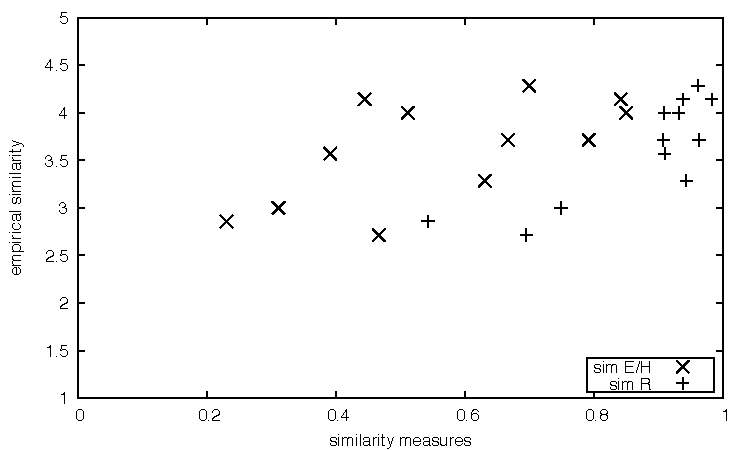
\includegraphics[width=0.6\textwidth]{../figures/visual-scatter.pdf}
\caption{Similarity measures and perceived similarity scatterplot}\label{fig:ci.scatter}
}
\end{figure}

\textbf{Analysis}. To test the assumption in \cref{eq:sim-assumption}, the relationship between the similarity measures and empirical similarity is analyzed.
Spearman's \(r_s\) is used on the median values of \(\mathfrak{S}\) and the similarity measures to show the required concordant (i.e.~positive monotonic) relationship.
There is a strong positive correlation between \(sim_{E/H}\) and \(\mathfrak{S}\) (\(r_s=0.7174\), (two-sided) \(p=0.0086\)) which is significant at \(\alpha=0.01\) even for the un-calibrated model with \(w_i=1\).
In contrast, the Tversky similarity \(sim_R\) does not exhibit a significant relationship.
Also, \(sim_{E/H}\) shows stronger differences between the \glspl{ui} compared to \(sim_R\), indicating that the Euclidean and Hamming formulations of similarity are a more suitable tool for \gls{Web Migration} purposes.
This can also be seen in \cref{fig:ci.scatter}.

Analysis of the empirical data shows rather low values for difficulty, which can be reasoned with the relatively simple user interfaces and the test subjects' proficiency with computers.
A moderate correlation between \(\text{Like}\) and \(\mathfrak{S}\) (\(r_s=0.5753\), \(p=0.0504\)) significant at \(\alpha=0.6\) was found, which can imply a preference for familiar interfaces.
The Like evaluation expectedly has the largest standard deviation (\(\sigma(\text{Like})=1.299\)) as it is the most subjective criterion.
Analyzing the influence of the three distances in pair-wise relations to \(\mathfrak{S}\), the following linear model was found highly significant at \(\alpha=0.001\) with good fit (\(p=0.001\), \(R^2=0.670\)): \(\mathfrak{S}=3.92 - 2.14 \text{dist}_{\text{ori}}\).

For the calibration process in \cref{sec:calibration}, a linear model is assumed.
We derive the weight factors from multiple linear regression of the three distances and the median of \(\mathfrak{S}\).
The resulting linear model in \cref{eq:calibrated-linear-model} is highly significant at \(\alpha = 0.001\) and has good fit (\(p=0.0001\), \(R^2=0.919\)).
The F-Test yields \(F=30.26\) which is \(F>f_{\text{crit}}\) with \(f_{\text{crit}}=15.83\) for \(p=0.001\), 3 degrees of freedom of the numerator and 8 degrees of freedom for the denominator, showing an improved model fit over the intercept-only model hypothesis.

\vspace{-30pt}
\begin{equation}\mathfrak{S}=4.61604 -3.24281\text{dist}_{\text{ori}} -1.27447\text{dist}_{\text{ord}} -0.888071\text{dist}_{\text{den}} + e[t] \label{eq:calibrated-linear-model}\end{equation}

\vspace{-15pt}
Using the factors of the distances as weights \(w_i\), the similarity measures can be re-calculated as shown in \cref{tbl:ci:sim-calibrated}.
The calibrated similarity measures \(sim_{E,\text{cal}}\) and \(sim_{H,\text{cal}}\) improve the correlation with median \(\mathfrak{S}\) to \(r_s=0.8383\), \(p=0.0007\), highly significant at \(\alpha = 0.001\).
\Cref{fig:ci.residuals} shows the results of residuals analysis with good overall alignment.
All variance inflation factors are less than \(\text{VIF}_{\text{den}} < 1.12\), showing a low multicollinearity of the distances' factors.
\Cref{tbl:ci:sim-calibrated} shows the calibrated similarity measures, and \cref{fig:ci.calibrated} visualizes the calibrated measures and their corresponding residuals QQ plots.

\hypertarget{tbl:ci:sim-calibrated}{}
\begin{longtable}[]{@{}llll@{}}
\caption[Calibrated \(sim\) measures]{\label{tbl:ci:sim-calibrated}Calibrated \(sim\) measures, maxima highlighted in bold}\tabularnewline
\toprule
UI & \(sim_{E,\text{cal}}\) & \(sim_{H,\text{cal}}\) & \(\overline{\mathfrak{S}}\)\tabularnewline
\midrule
\endfirsthead
\toprule
UI & \(sim_{E,\text{cal}}\) & \(sim_{H,\text{cal}}\) & \(\overline{\mathfrak{S}}\)\tabularnewline
\midrule
\endhead
\(u'_1\) & 0,9088 & 0,8999 & 4\tabularnewline
\(u''_{1,\text{ori}}\) & 0,5430 & 0,4726 & 2.8571\tabularnewline
\(u''_{1,\text{ord}}\) & \textbf{0,9611} & \textbf{0,945} & \textbf{4.2857}\tabularnewline
\(u''_{1,\text{den}}\) & 0,9074 & 0,8906 & 3.7143\tabularnewline
\(u'_2\) & \textbf{0,9822} & \textbf{0,9822} & \textbf{4.1429}\tabularnewline
\(u''_{2,\text{ori}}\) & 0,7487 & 0,6904 & 3\tabularnewline
\(u''_{2,\text{ord}}\) & 0,9431 & 0,9282 & 3.2857\tabularnewline
\(u''_{2,\text{den}}\) & 0,9093 & 0,8719 & 3.5714\tabularnewline
\(u'_3\) & \textbf{0,9627} & \textbf{0,9627} & 3.7143\tabularnewline
\(u''_{3,\text{ori}}\) & 0,6952 & 0,6602 & 2.7143\tabularnewline
\(u''_{3,\text{ord}}\) & 0,9311 & 0,9048 & 4\tabularnewline
\(u''_{3,\text{den}}\) & 0,9378 & 0,9378 & \textbf{4.1429}\tabularnewline
\bottomrule
\end{longtable}
\pagebreak

\begin{figure}[h]
\centering

\subfloat[Residual Density Plot]{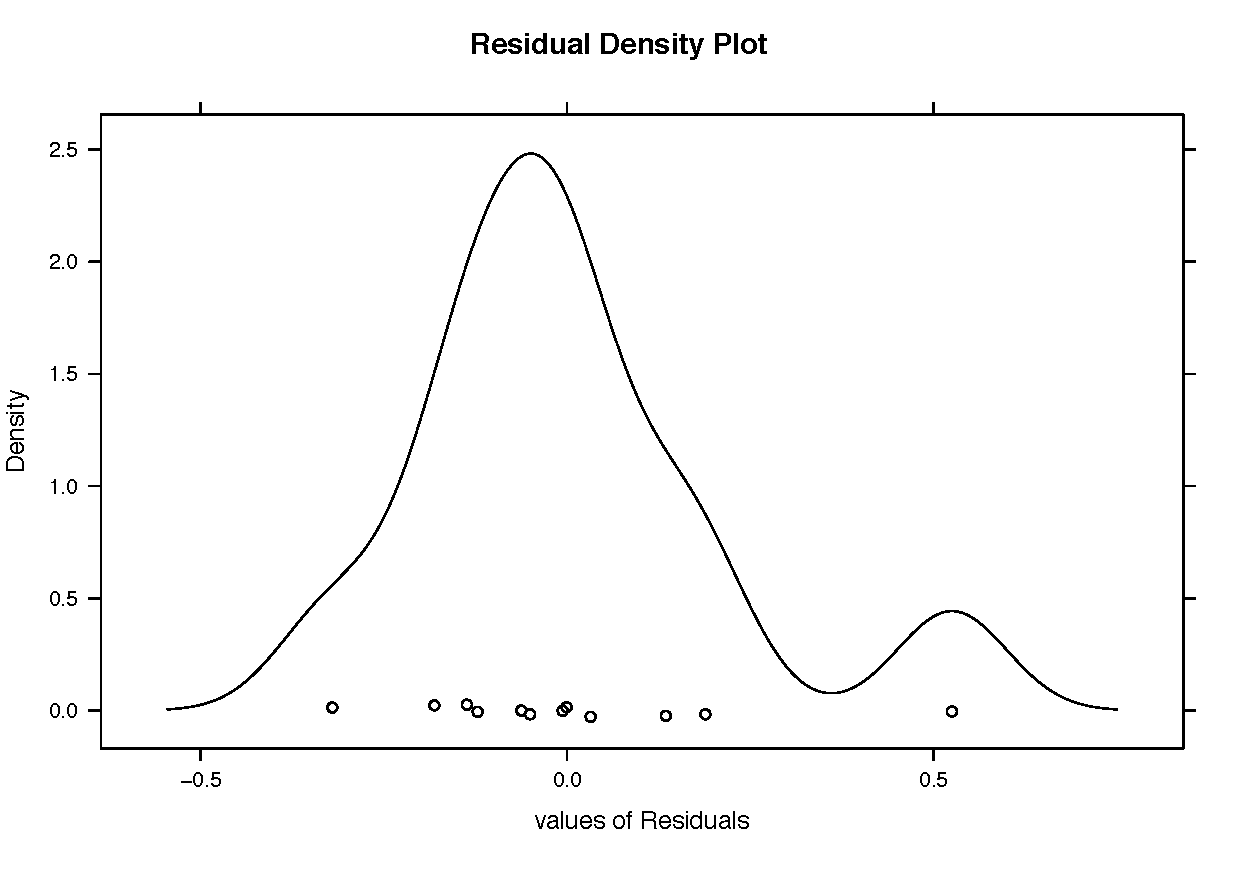
\includegraphics[width=0.49\textwidth]{../figures/visual-residuals-density.pdf}\label{fig:residuals-a}}
\subfloat[QQ Plot of Residuals]{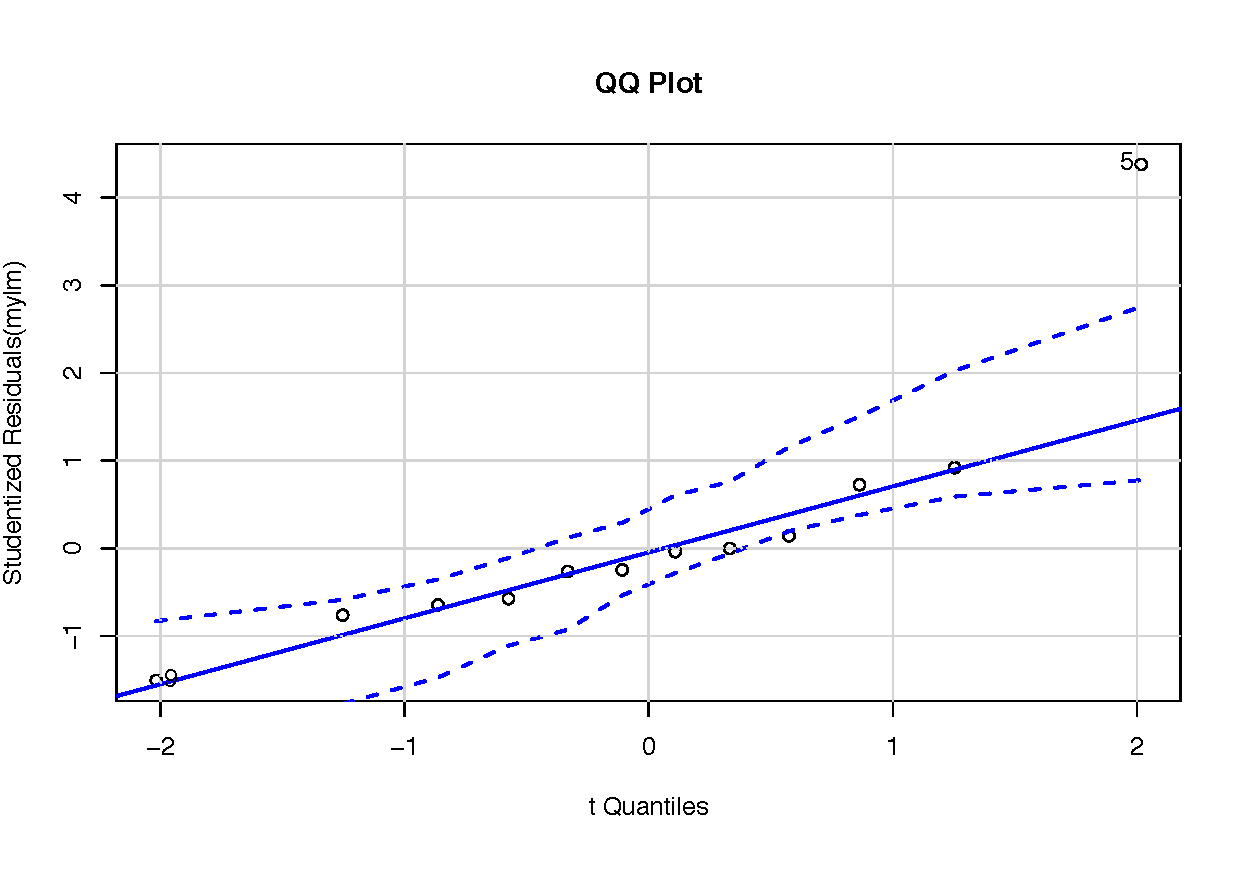
\includegraphics[width=0.49\textwidth]{../figures/visual-residuals-qq.pdf}\label{fig:residuals-b}}

\caption[Residual Plots]{Residual Plots, created using \autocite{Wessa2017Statistics}}

\label{fig:ci.residuals}

\end{figure}

\begin{figure}[h]
\centering

\subfloat[\(sim_{E,\text{cal}}\)]{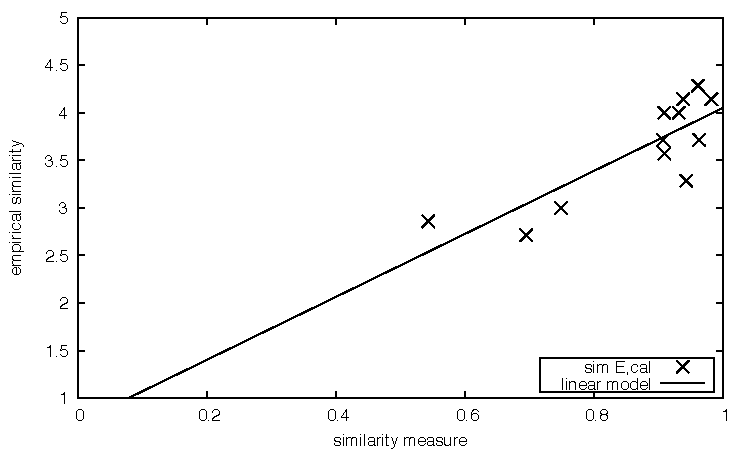
\includegraphics[width=0.49\textwidth]{../figures/visual-calibrated-e2.pdf}\label{fig:calibrated-e2}}
\subfloat[\(sim_{H,\text{cal}}\)]{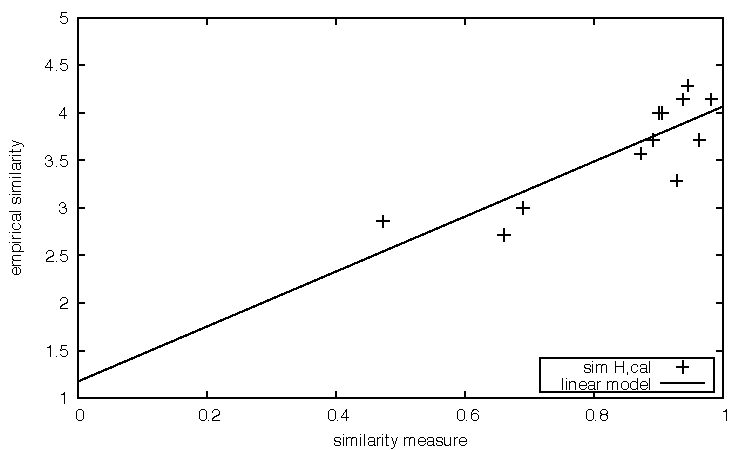
\includegraphics[width=0.49\textwidth]{../figures/visual-calibrated-h2.pdf}\label{fig:calibrated-h2}}

\subfloat[\(sim_{E,\text{cal}}\) Residuals QQ Plot]{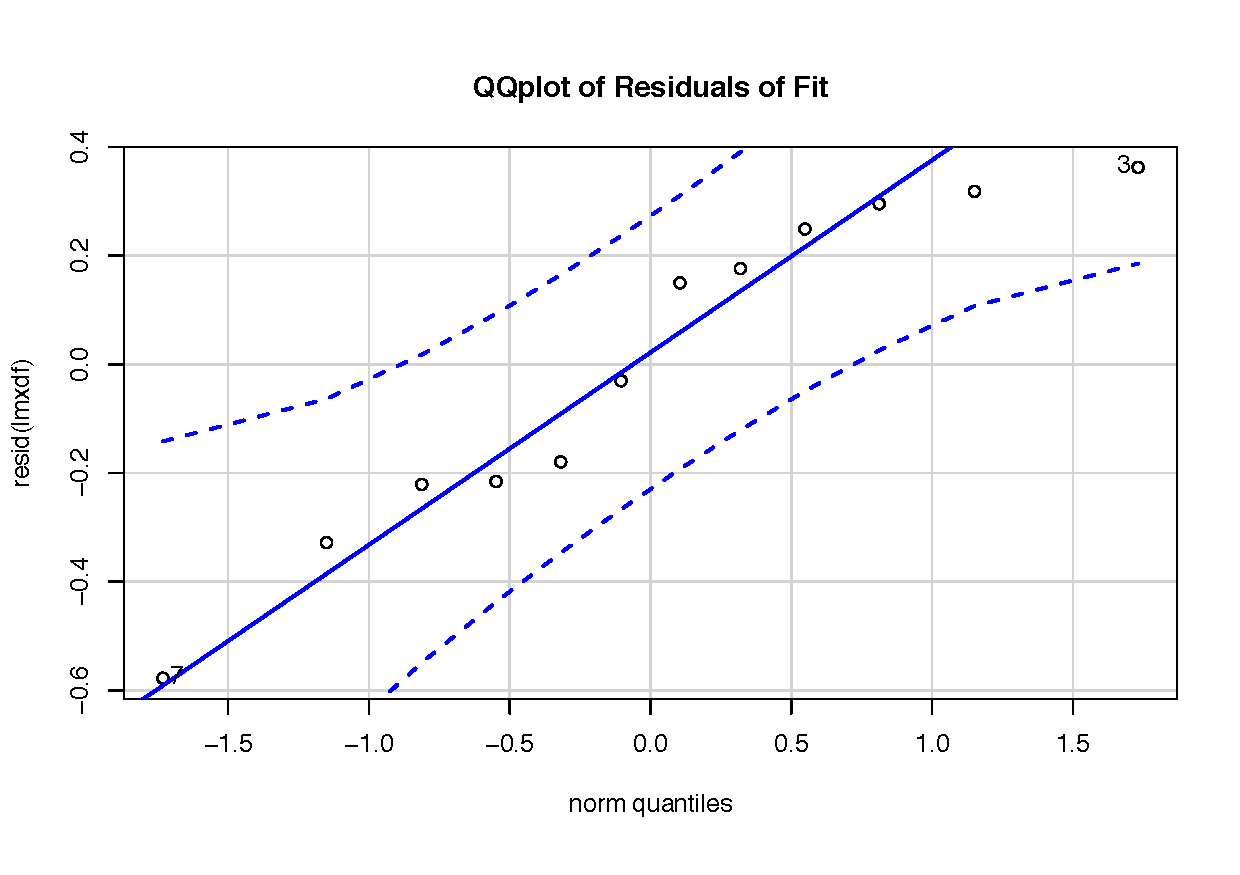
\includegraphics[width=0.49\textwidth]{../figures/visual-calibrated-residuals-e2.pdf}\label{fig:calibrated-residuals-e2}}
\subfloat[\(sim_{H,\text{cal}}\) Residuals QQ Plot]{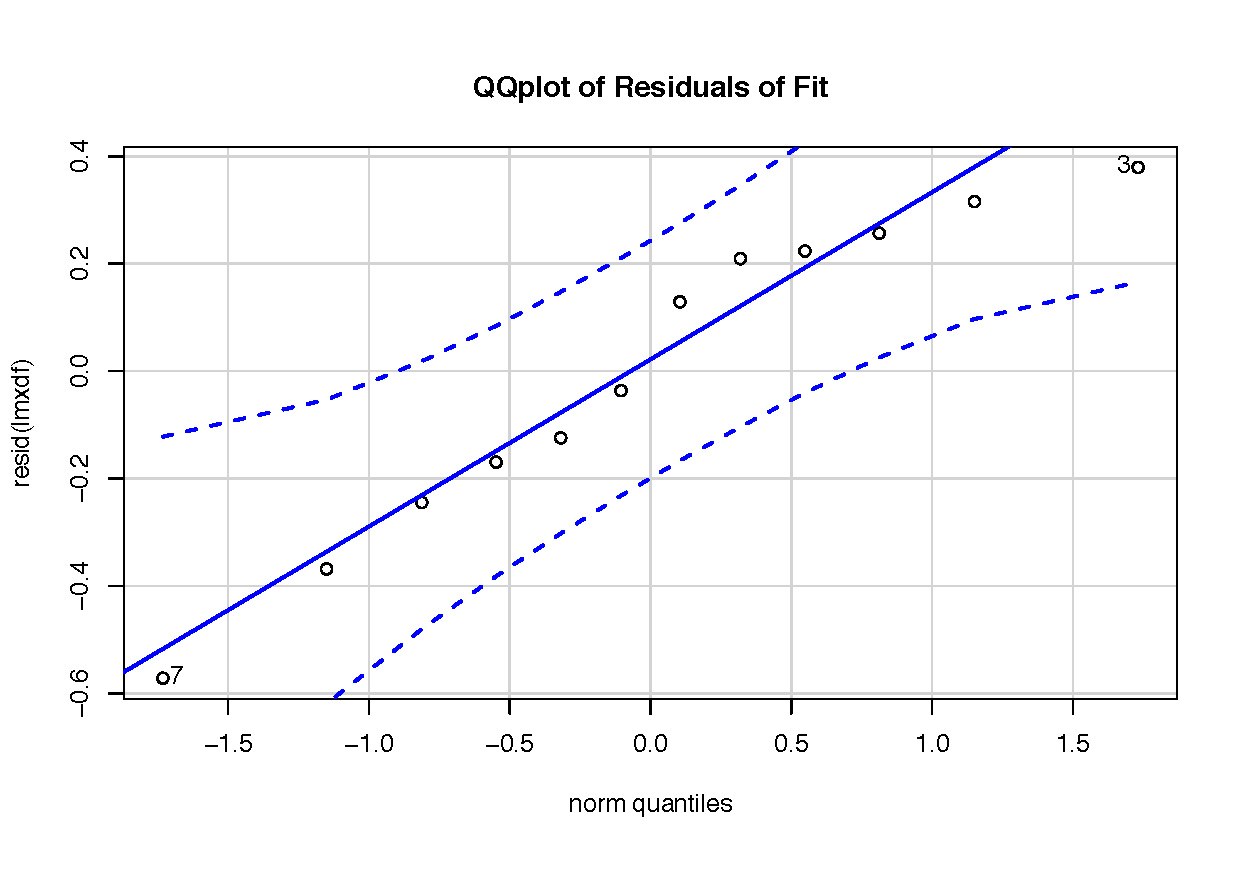
\includegraphics[width=0.49\textwidth]{../figures/visual-calibrated-residuals-h2.pdf}\label{fig:calibrated-residuals-h2}}

\caption[Calibrated Similarity Measures and Residuals QQ plots]{Calibrated Similarity Measures and Residuals QQ plots,\\ created using \autocite{Wessa2017Statistics}}

\label{fig:ci.calibrated}

\end{figure}

\textbf{Threats to Validity}. \emph{Construct validity} of this experiment is threatened by possible variations in the evaluation runs.
This was addressed by providing a fixed environment: All sessions were performed on the same PC and screen in order to ensure consistent visual representation and interaction across all test subjects.
The task list \(T_i\) ensured that all test subjects solved the same tasks on the user interfaces and thus had the same understanding of the underlying Task and Behavior models.
The tasks were designed as small and self-contained interactions that did not allow for alternative interaction paths.
All test subjects received the same introduction and demonstration of the tasks on the \glslink{Legacy System}{legacy} user interface.
The second important aspect affecting construct validity is the analysis of Likert items in the questionnaire.
In the context of discussions about limitations of valid statistical measures on ordinal-scaled Likert items, \cref{tbl:ci:sim} follows the practical approach commonly used in the \gls{hci} field and user research to apply mean as it better supports smaller sample sizes \autocite{Sauro2016}.
However, all interpretations are restricted to ordinal statements; no interval or ratio statements are derived.
The correlation analysis was conducted on the median values using Spearman's \(r_s\) instead of Pearson's \(\rho\) for the same reason.

\emph{Internal validity} of this experiment is threatened through potential subjective biases.
In order to avoid participants being biased towards giving higher ratings to the ``original'' \glspl{wui} from \(U_W\) in comparison to the variations in \(U_V\), we assigned identifiers not disclosing this information (\(u'_1 \widehat{=} A3\), \(u'_2\widehat{=} B2\), and \(u'_3\widehat{=} C2\)).
Also, the order in which \gls{web} versions of the same \glslink{Legacy System}{legacy} \gls{ui} were evaluated was randomized to avoid bias through test subjects adjusting to the same sequence of interfaces.
The test subjects' preference for similar interfaces observed in the \(\text{Like}\) evaluations may have been affected by the experiment, hinting that similar equals good.
However, we measured this data only as additional information and did not perform further detailed analysis, as the overall preference for similar interfaces through migration has already been well-researched in previous studies.
It can be argued that the similarity evaluations of the test subjects are highly subjective.
However, this is intended since the measured item, the perceived similarity of \glspl{ui}, is a subjective notion.
This is addressed by the model creation and calibration process, and the good model fit has shown applicability.

\emph{External validity} of the experiment is threatened through limitations in the generalizability of results.
Evidently, the evaluation results cannot be used as a generalized ready-made model for \gls{ui} Similarity in arbitrary \gls{Web Migration} contexts, as the similarity evaluations of the test subjects are highly subjective.
However, AWSM:CI aims at providing a strategy for creating and adapting a similarity measurement model tailored for a specific target user group of a specific \gls{Legacy System} to be migrated to the \gls{web}.
In that way, the evaluation experiment has shown that the AWSM:CI method can be successfully applied to achieve this result, without making claims with regards to the generalisability of the concrete numerical results and derived findings.

\textbf{Conclusion of AWSM:CI experimentation}. The AWSM:CI evaluation experiment has shown that the similarity measures based on Tversky distances in the Orientation, Order, and Density dimensions of layout similarity can be effectively used to estimate the perceived similarity of the user interface in \gls{Web Migration}.
Of the three similarity measures, the Euclidean formulation \(sim_E\) and the Hamming formulation \(sim_H\) are better applicable than the Tversky mode formulation \(sim_R\).
Both similarity measures in their initial state (all weights set to one) fulfill the required concordance assumption.
It was shown that the AWSM:CI calibration process conducted with only limited effort, i.e.~seven users from the target group and three user interfaces with three variations, can be applied to improve the initial similarity measures to an \(R^2=0.919\) fit on perceived similarity, highly significant with \(p=0.0001\).
Different influences of the proposed distances were observed: while Density was found to be the most influenced by changes in other dimensions and having only small influence on similarity, Orientation showed stronger impact.
The concrete findings on differences in the influence of the distances have to be seen in the light of a relatively small group of test users and cannot be generalized.
However, AWSM:CI calibration can be applied in order to adjust this to specific target user groups and analyze concrete preferences within these groups.
The efficiency of AWSM:CI is evident when comparing to the naive approach of a traditional full empirical evaluation of similarity of all different variations of migrated \gls{web} \glspl{ui} with test subjects.
Instead, AWSM:CI provides a method for automated computation of similarity measures as approximation of perceived similarity.
These measures can be tailored to the target group with a limited effort calibration process on a small group of representatives from the target group.

\vspace{-10pt}
\hypertarget{sec:ci.evaluation.objective}{%
\subsection{Research Results}\label{sec:ci.evaluation.objective}}
\vspace{10pt}

The research objective addressed by this chapter, \cref{ro:3}, to enable control of the impact of user interface changes through \gls{Web Migration} on customers with limited resources and lack of \gls{Web Engineering} expertise, is achieved.
The effectiveness, applicability, and calibratability of the AWSM:CI Method for measuring Visual \gls{ui} Similarity of \legacy and \gls{web}-migrated user interfaces have been demonstrated and detailed through experimentation.
Efficiency of AWSM:CI is currently only half-satisfied due to limitations in the quality of fully automated \gls{ui} Element detection.
However, the overall feasibility of the automation approach could be demonstrated.
Expertise requirements are limited through the computable similarity measures, automation, and calibration artifacts and strategy presented above.
In spite of the half-restricted efficiency results, \cref{ro:3} is considered as achieved.
AWSM:CI RQ1 was answered through the \gls{ui} similarity technique introduced in \cref{sec:visual-analysis}.
AWSM:CI RQ2 was answered through specification of a vision-based approach for Similarity Analysis, enabling application on both \legacy and \webbased user interfaces, as defined in \cref{sec:visual-analysis.overview}.
AWSM:CI RQ3 was answered through the realization of \gls{ui} Similarity Aanalysis by distance-based computable measures in \cref{sec:computing-sim} and specifying a solution for automatic detection of \gls{ui} Elements in \cref{sec:segmentation}.

\hypertarget{sec:ci.summary}{%
\section{Summary}\label{sec:ci.summary}}
\vspace{15pt}

This chapter presented the \gls{awsm} Customer Impact method, which facilitates the measurement and control of visible change in user interfaces by \gls{Web Migration}, specifying a novel \gls{ui} Similarity measurement strategy that can be calibrated to the target user group.
The strategy is supported through a computer-vision based \gls{ui} Element detection and computation of \gls{ui} layout distances from visual analysis.
The conceptual model of the AWSM:CI techniques and their implementation in the Toolsuite have been described.
In the evaluation, we have shown the feasibility of the approach and the quality of its measurements with limited effort, improvement of the measurements through calibration, and how to avoid extensive empirical evaluations with only a small number of users.
Furthermore, the experiments provided insights on influence factors on perceived similarity contributing to ongoing research in this field.
While this research is still in early stages, operationalization of the proposed similarity measure can help controlling customer impact in \gls{Web Migration}.
